%% Преамбула TeX-файла

% 1. Стиль и язык
\documentclass[utf8x, 12pt]{G7-32} % Стиль (по умолчанию будет 14pt)

% Остальные стандартные настройки убраны в preamble.inc.tex.
\sloppy

% Настройки стиля ГОСТ 7-32
% Для начала определяем, хотим мы или нет, чтобы рисунки и таблицы нумеровались в пределах раздела, или нам нужна сквозная нумерация.
\EqInChapter % формулы будут нумероваться в пределах раздела
\TableInChapter % таблицы будут нумероваться в пределах раздела
\PicInChapter % рисунки будут нумероваться в пределах раздела
\usepackage{slashbox}

% Добавляем гипертекстовое оглавление в PDF
\usepackage[
bookmarks=true, colorlinks=true, unicode=true,
urlcolor=black,linkcolor=black, anchorcolor=black,
citecolor=black, menucolor=black, filecolor=black,
]{hyperref}

% Изменение начертания шрифта --- после чего выглядит таймсоподобно.
% apt-get install scalable-cyrfonts-tex

\IfFileExists{cyrtimes.sty}
    {
        \usepackage{cyrtimespatched}
    }
    {
        % А если Times нету, то будет CM...
    }

\usepackage{graphicx}   % Пакет для включения рисунков

% С такими оно полями оно работает по-умолчанию:
% \RequirePackage[left=20mm,right=10mm,top=20mm,bottom=20mm,headsep=0pt]{geometry}

\geometry{right=20mm}
\geometry{left=30mm}


% Пакет Tikz
\usepackage{tikz}
\usetikzlibrary{arrows,positioning,shadows}
\usepackage{pgfplots}

% Произвольная нумерация списков.
\usepackage{enumerate}

% ячейки в несколько строчек
\usepackage{multirow}

% itemize внутри tabular
\usepackage{paralist,array}

% Центрирование подписей к плавающим окружениям
\usepackage[justification=centering]{caption}

% My

\usepackage[export]{adjustbox}
\usepackage{float}

\usepackage{subcaption}
\usepackage{comment}
\usepackage{tabularx}





%%
\usepackage{ifthen}
\usepackage{url}
\usepackage{listings}
\usepackage{rotating}
\usepackage{afterpage}

%% caption less table to specify restful primitives
\newcommand{\restful}[1]
{
	\begin{center}
		\begin{tabular}{l p{12cm}}
			\hline
			#1
			\hline
		\end{tabular}
	\end{center}
	\vspace{6pt}
}


%% caption less table to specify restful uri
\newcommand{\routes}[1]
{
	\begin{center}
		\begin{tabular}{p{\textwidth}}
			\hline
			#1
			\hline
		\end{tabular}
	\end{center}
	\vspace{6pt}
}
%
%
%

\newcommand{\mimetype}[2]{#1 & #2 \\\noalign{\smallskip}}
\newcommand{\head}[2]{#1 & #2 \\\noalign{\smallskip}}
\newcommand{\uri}[2]{\url{#1} \\ #2 \vspace{8pt} \\\noalign{\smallskip}}
\newcommand{\env}[2]{#1 & #2 \\\noalign{\smallskip}}
%

%%% resource definition table
\newcommand{\resource}[1]
{
	\begin{center}
		\begin{tabular}{l l p{12cm}}
			\hline
			#1
			\hline
		\end{tabular}
	\end{center}
	\vspace{6pt}
}
\newcommand{\attr}[3]{{\tt #1} & #2 & #3 \\\noalign{\smallskip}}

%
%
\newcommand{\request}[6]
{
	\begin{center}
		\begin{tabular}{l p{12cm}}
			\hline
			Метод:  & #1 \url{#2} \\\noalign{\smallskip}
			& #3     \vspace{4pt}\\ 
			Запрос:  & #4 \vspace{4pt}\\
			Ответ:  & #5 \vspace{4pt}\\
			Статус:   & #6 \\
			\hline
		\end{tabular}
	\end{center}
	\vspace{6pt}
}

\newcommand{\sep}{\\\noalign{\smallskip} &}

\newcommand{\status}[1]
{
	\ifthenelse{\equal{#1}{100}}{100 Continue}{}%
	\ifthenelse{\equal{#1}{101}}{101 Switching Protocols}{}%
	\ifthenelse{\equal{#1}{200}}{200 OK}{}%
	\ifthenelse{\equal{#1}{201}}{201 Created}{}%
	\ifthenelse{\equal{#1}{202}}{202 Accepted}{}%
	\ifthenelse{\equal{#1}{203}}{203 Non-Authoritative Information}{}%
	\ifthenelse{\equal{#1}{204}}{204 No Content}{}%
	\ifthenelse{\equal{#1}{205}}{205 Reset Content}{}%
	\ifthenelse{\equal{#1}{206}}{206 Partial Content}{}%
	\ifthenelse{\equal{#1}{300}}{300 Multiple Choices}{}%
	\ifthenelse{\equal{#1}{301}}{301 Moved Permanently}{}%
	\ifthenelse{\equal{#1}{302}}{302 Found}{}%
	\ifthenelse{\equal{#1}{303}}{303 See Other}{}%
	\ifthenelse{\equal{#1}{304}}{304 Not Modified}{}%
	\ifthenelse{\equal{#1}{307}}{307 Temporary Redirect}{}%
	\ifthenelse{\equal{#1}{302}}{302 Found}{}%
	\ifthenelse{\equal{#1}{400}}{400 Bad Request}{}%
	\ifthenelse{\equal{#1}{401}}{401 Unauthorized}{}%
	\ifthenelse{\equal{#1}{402}}{402 Payment Required}{}%
	\ifthenelse{\equal{#1}{403}}{403 Forbidden}{}%
	\ifthenelse{\equal{#1}{404}}{404 Not Found}{}%
	\ifthenelse{\equal{#1}{405}}{405 Method Not Allowed}{}%
	\ifthenelse{\equal{#1}{406}}{406 Not Acceptable}{}%
	\ifthenelse{\equal{#1}{407}}{407 Proxy Authentication Required}{}%
	\ifthenelse{\equal{#1}{408}}{408 Request Timeout}{}%
	\ifthenelse{\equal{#1}{409}}{409 Conflict}{}%
	\ifthenelse{\equal{#1}{410}}{410 Gone}{}%
	\ifthenelse{\equal{#1}{411}}{411 Length Required}{}%
	\ifthenelse{\equal{#1}{412}}{412 Precondition Failed}{}%
	\ifthenelse{\equal{#1}{413}}{413 Request Entity Too Large}{}%
	\ifthenelse{\equal{#1}{414}}{414 Request-URI Too Long}{}%
	\ifthenelse{\equal{#1}{415}}{415 Unsupported Media Type}{}%
	\ifthenelse{\equal{#1}{416}}{416 Requested Range Not Satisfiable}{}%
	\ifthenelse{\equal{#1}{417}}{417 Expectation Failed}{}%
	\ifthenelse{\equal{#1}{422}}{422 Unprocessable Entity}{}%
	\ifthenelse{\equal{#1}{500}}{500 Internal Server Error}{}%
	\ifthenelse{\equal{#1}{501}}{501 Not Implemented}{}%
	\ifthenelse{\equal{#1}{502}}{502 Bad Gateway}{}%
	\ifthenelse{\equal{#1}{503}}{503 Service Unavailable}{}%
	\ifthenelse{\equal{#1}{504}}{504 Gateway Timeout}{}%
	\ifthenelse{\equal{#1}{505}}{505 HTTP Version Not Supported}{}%
}

\newcommand{\httpcode}[2]{\status{#1} & #2 \\\noalign{\smallskip}}

\newcommand{\example}[1]{\noindent {\bf #1}}


% Настройки листингов.
\ifPDFTeX
% Листинги

\usepackage{listings}
\usepackage{wrapfig}
% Значения по умолчанию
\lstset{
  basicstyle= \footnotesize,
  breakatwhitespace=true,% разрыв строк только на whitespacce
  breaklines=true,       % переносить длинные строки
%   captionpos=b,          % подписи снизу -- вроде не надо
  inputencoding=koi8-r,
  numbers=left,          % нумерация слева
  numberstyle=\footnotesize,
  showspaces=false,      % показывать пробелы подчеркиваниями -- идиотизм 70-х годов
  showstringspaces=false,
  showtabs=false,        % и табы тоже
  stepnumber=1,
  tabsize=4,              % кому нужны табы по 8 символов?
  frame=single,
  escapeinside={(*}{*)}, %выделение
  literate={а}{{\selectfont\char224}}1
  {б}{{\selectfont\char225}}1
  {в}{{\selectfont\char226}}1
  {г}{{\selectfont\char227}}1
  {д}{{\selectfont\char228}}1
  {е}{{\selectfont\char229}}1
  {ё}{{\"e}}1
  {ж}{{\selectfont\char230}}1
  {з}{{\selectfont\char231}}1
  {и}{{\selectfont\char232}}1
  {й}{{\selectfont\char233}}1
  {к}{{\selectfont\char234}}1
  {л}{{\selectfont\char235}}1
  {м}{{\selectfont\char236}}1
  {н}{{\selectfont\char237}}1
  {о}{{\selectfont\char238}}1
  {п}{{\selectfont\char239}}1
  {р}{{\selectfont\char240}}1
  {с}{{\selectfont\char241}}1
  {т}{{\selectfont\char242}}1
  {у}{{\selectfont\char243}}1
  {ф}{{\selectfont\char244}}1
  {х}{{\selectfont\char245}}1
  {ц}{{\selectfont\char246}}1
  {ч}{{\selectfont\char247}}1
  {ш}{{\selectfont\char248}}1
  {щ}{{\selectfont\char249}}1
  {ъ}{{\selectfont\char250}}1
  {ы}{{\selectfont\char251}}1
  {ь}{{\selectfont\char252}}1
  {э}{{\selectfont\char253}}1
  {ю}{{\selectfont\char254}}1
  {я}{{\selectfont\char255}}1
  {А}{{\selectfont\char192}}1
  {Б}{{\selectfont\char193}}1
  {В}{{\selectfont\char194}}1
  {Г}{{\selectfont\char195}}1
  {Д}{{\selectfont\char196}}1
  {Е}{{\selectfont\char197}}1
  {Ё}{{\"E}}1
  {Ж}{{\selectfont\char198}}1
  {З}{{\selectfont\char199}}1
  {И}{{\selectfont\char200}}1
  {Й}{{\selectfont\char201}}1
  {К}{{\selectfont\char202}}1
  {Л}{{\selectfont\char203}}1
  {М}{{\selectfont\char204}}1
  {Н}{{\selectfont\char205}}1
  {О}{{\selectfont\char206}}1
  {П}{{\selectfont\char207}}1
  {Р}{{\selectfont\char208}}1
  {С}{{\selectfont\char209}}1
  {Т}{{\selectfont\char210}}1
  {У}{{\selectfont\char211}}1
  {Ф}{{\selectfont\char212}}1
  {Х}{{\selectfont\char213}}1
  {Ц}{{\selectfont\char214}}1
  {Ч}{{\selectfont\char215}}1
  {Ш}{{\selectfont\char216}}1
  {Щ}{{\selectfont\char217}}1
  {Ъ}{{\selectfont\char218}}1
  {Ы}{{\selectfont\char219}}1
  {Ь}{{\selectfont\char220}}1
  {Э}{{\selectfont\char221}}1
  {Ю}{{\selectfont\char222}}1
  {Я}{{\selectfont\char223}}1
}

% Стиль для псевдокода: строчки обычно короткие, поэтому размер шрифта побольше
\lstdefinestyle{pseudocode}{
  basicstyle=\small,
  keywordstyle=\color{black}\bfseries\underbar,
  language=Pseudocode,
  numberstyle=\footnotesize,
  commentstyle=\footnotesize\it
}

% Стиль для обычного кода: маленький шрифт
\lstdefinestyle{realcode}{
  basicstyle=\scriptsize,
  numberstyle=\footnotesize
}

% Стиль для коротких кусков обычного кода: средний шрифт
\lstdefinestyle{simplecode}{
  basicstyle=\footnotesize,
  numberstyle=\footnotesize
}

% Стиль для BNF
\lstdefinestyle{grammar}{
  basicstyle=\footnotesize,
  numberstyle=\footnotesize,
  stringstyle=\bfseries\ttfamily,
  language=BNF
}

% Определим свой язык для написания псевдокодов на основе Python
\lstdefinelanguage[]{Pseudocode}[]{Python}{
  morekeywords={each,empty,wait,do},% ключевые слова добавлять сюда
  morecomment=[s]{\{}{\}},% комменты {а-ля Pascal} смотрятся нагляднее
  literate=% а сюда добавлять операторы, которые хотите отображать как мат. символы
    {->}{\ensuremath{$\rightarrow$}~}2%
    {<-}{\ensuremath{$\leftarrow$}~}2%
    {:=}{\ensuremath{$\leftarrow$}~}2%
    {<--}{\ensuremath{$\Longleftarrow$}~}2%
}[keywords,comments]

% Свой язык для задания грамматик в BNF
\lstdefinelanguage[]{BNF}[]{}{
  morekeywords={},
  morecomment=[s]{@}{@},
  morestring=[b]",%
  literate=%
    {->}{\ensuremath{$\rightarrow$}~}2%
    {*}{\ensuremath{$^*$}~}2%
    {+}{\ensuremath{$^+$}~}2%
    {|}{\ensuremath{$|$}~}2%
}[keywords,comments,strings]

% Подписи к листингам на русском языке.
\renewcommand\lstlistingname{\cyr\CYRL\cyri\cyrs\cyrt\cyri\cyrn\cyrg}
\renewcommand\lstlistlistingname{\cyr\CYRL\cyri\cyrs\cyrt\cyri\cyrn\cyrg\cyri}

\else
\usepackage{local-minted}
\fi

% Полезные макросы листингов.
% Любимые команды
\newcommand{\Code}[1]{\textbf{#1}}


\begin{document}

\frontmatter % выключает нумерацию ВСЕГО; здесь начинаются ненумерованные главы: реферат, введение, глоссарий, сокращения и прочее.

% Команды \breakingbeforechapters и \nonbreakingbeforechapters
% управляют разрывом страницы перед главами.
% По-умолчанию страница разрывается.

% \nobreakingbeforechapters
% \breakingbeforechapters

% Также можно использовать \Referat, как в оригинале
%\begin{abstract}
%	Титульный лист. Эта страница нужна мне, чтобы не сбивалась нумерация страниц
%	\cite{Dh}
%	\cite{Bayer}
%	\cite{Habr1}
%	\cite{Noise_func}
%	\cite{Ulich}

%Это пример каркаса расчётно-пояснительной записки, желательный к использованию в РПЗ проекта по курсу РСОИ.

%Данный опус, как и более новые версии этого документа, можно взять по адресу (\url{https://github.com/rominf/latex-g7-32}).

%\end{abstract}
% НАЧАЛО ТИТУЛЬНОГО ЛИСТА
\begin{center}
	\bigbreak
	\textit{
		Государственное образовательное учреждение высшего профессионального образования}\\ 
	
	\textit{
		\noindent
		\begin{minipage}{0.2\textwidth}% adapt widths of minipages to your needs
			
\includegraphics[scale=0.5]{img/bmstu-logo.png}~
		\end{minipage}
		\hfill
		\begin{minipage}{0.7\textwidth}\centering
		    \bf  «Московский государственный технический университет\\ 
			\bf имени Н. Э. Баумана»\\
			\bf (МГТУ им. Н.Э. Баумана)\\
		\end{minipage}
		\bigbreak
	}
	
	\noindent\rule{\textwidth}{2pt}
	\bigbreak
	

	\noindent
	\begin{minipage}{0.15\textwidth}\raggedright
		ФАКУЛЬТЕТ\\
		КАФЕДРА
	\end{minipage}
	\hfill
	\begin{minipage}{0.8\textwidth}\centering
		«Информатика и системы управления»\\
		«Программное обеспечение ЭВМ и информационные технологии»
	\end{minipage}
	
	\vspace{\fill}
	\normalsize{\bf Р А С Ч Ё Т Н О - П О Я С Н И Т Е Л Ь Н А Я\space\space З А П И С К А}\\
	\normalsize{\bf к курсовой работе на тему:}\\
	\large{<<>>}\\\vspace{\fill}	
	\normalsize {
		\noindent
		\makebox[0pt][l]{Студент}%
		\makebox[\textwidth][c]{}%
		\makebox[0pt][r]{{$\underset{\text{(Подипсь, дата)}}{\underline{\hspace{6cm}}}$ \space\space\space Анисимов Н.С.}}
	}\\
	\bigbreak	
	\normalsize {
		\noindent
		\makebox[0pt][l]{Руководитель курсового проекта}%
		\makebox[\textwidth][c]{ ~~~~~~~~      }%
		\makebox[0pt][r]{{$\underset{\text{(Подпись, дата)}}{\underline{\hspace{6cm}}}$ \space Строганов Ю.В.}}
	}
\end{center}
\vspace{\fill}
\begin{center} Москва 2017 \end{center}

\thispagestyle{empty} % 
% КОНЕЦ ТИТУЛЬНОГО ЛИСТА


%%% Local Variables: 
%%% mode: latex
%%% TeX-master: "rpz"
%%% End: 

\tableofcontents

\Introduction

В настоящие время все чаще для проведения тестирования используются автоматические системы. Многочисленные олимпиады проводятся на базе онлайн-тестов. Такие организации как Яндекс, Mail.ru, Stepik, предоставляют свои средства автоматического тестирования, что подтверждает актуальность разработки подобных систем.

\mainmatter % это включает нумерацию глав и секций в документе ниже

\chapter{ Аналитический раздел }

\section{Существующий системы автоматического тестирования}

\section{Базы данных}
Согласно концепции баз данных, основой информационных технологий являются данные, которые должны быть организованы в базы данных в целях адекватного отображения изменяющегося реального мира и удовлетворения информационных потребностей пользователей. Одним из важнейших понятий в теории баз данных является понятие информации. Информация - это любые сведения о каком-либо событии, процессе, объекте. К информации может относиться все, что может интересовать пользователя любого уровня.

Данные -- это информация, представленная в определенном виде, позволяющем автоматизировать её сбор, хранение и дальнейшую обработку человеком или информационным средством. Для компьютерных технологий данные -- это информация в дискретном, фиксированном виде, удобная для хранения, обработки на ЭВМ, а также для передачи по каналам связи. 

База данных (БД) - именованная совокупность данных, отражающая состояние объектов и их отношений в рассматриваемой предметной области, иными словами БД - это совокупность взаимосвязанных данных при такой минимальной избыточности, которая допускает их использование оптимальным образом для одного или нескольких приложений в определенной предметной области.

Важнейшие свойства баз данных:
\begin{itemize}
\item Целостность. В каждый момент времени существования БД сведения, содержащиеся в ней, должны быть непротиворечивы. Например, необходимо отслеживать диапазон допустимых значений, соотношения между значениями в полях, особенности написания формата. Существуют ограничения, работающие только при удалении записей. Например, нельзя удалять запись, связанную с другой неудаляемой записью.
\item Восстанавливаемость предполагает возможность восстановления БД после сбоя системы или отдельных видов порчи системы. Сюда относится проверка наличия файлов, составляющих приложение. В основном свойство восстанавливаемости обеспечивается дублированием БД и использованием техники повышенной надежности.
\item Безопасность БД предполагает защиту данных от преднамеренного и непреднамеренного доступа, модификации или разрушения. Применяется запрещение несанкционированного доступа, защита от копирования и криптографическая защита. Также необходимы и чисто административные меры, например ограничение доступа к носителям информации. 
\item Эффективность обычно понимается как:
\begin{itemize}
\item  минимальное время реакции на запрос пользователя;
\item  минимальные потребности в памяти;
\item  сочетание этих параметров.
\end{itemize}
\item Предельные размеры и эксплуатационные ограничения, накладываемые использованием данной БД, могут существенно повлиять на проектное решение.
\end{itemize}
Создание баз данных, поддержка их в целостном, непротиворечивом состоянии, обеспечение безопасности их использования и сохранности информации вплоть до восстановления её после различных сбоев, предоставление различных информационных услуг пользователям и многое другое обеспечивается СУБД.

Термин СУБД включает в себя довольно большое количество сильно отличающихся друг от друга инструментов для работы с базами данных (отдельные программы и подключаемые библиотеки). Так как данные бывают различных видов и типов, начиная со второй половины 20 века было разработано огромное количество разных СУБД и других приложений для работы с БД.

СУБД основываются на модели базы данных - это специальные структуры предназначенные для работы с данными. Все СУБД сильно отличаются в том, каким образом они хранят и обрабатывают свои данные.

В модели данных различают три главные составляющие:
\begin{itemize}
	\item структурная часть, определяющая правила порождения допустимых для данной СУБД видов структур данных.
	\item управляющая часть, определяющая возможные операции над такими структурами.
	\item классы ограничений целостности данных, которые могут быть реализованы средствами этой системы.
\end{itemize}


Каждая система поддерживает различные модели и структуры баз данных. Эта модель и определяет, как создаваемая СУБД будет оперировать данными. Существует довольно немного моделей БД, которые предоставляют способы четкого структурирования данных, самая популярная из таких моделей - реляционная модель.
Реляционная модель и реляционные БД могут быть очень мощным инструментом, но только если программист знает как с ними обращаться. Недавно, стали набирать популярность NoSQL системы с обещанием избавиться от старых проблем БД и добавить новый функционал. Исключая жесткую структуру данных, при этом сохранив реляционный стиль, эти СУБД предлагают более свободный способ работы с ними и гораздо большие возможности для их настройки. Хотя не обходится и без возникновения новых проблем.

\subsection{Реляционная модель}
Реляционный (SQL) подход обозначает определенную идеологию создания баз данных.

Во-первых, БД представляется на внешнем, не зависящем от структуры ЭВМ уровне в виде совокупности двумерных таблиц, повседневно встречающихся в человеческой практике. Работа с таблицами привычна и понятна каждому пользователю. Поиск и обработка информации, хранящейся в таблицах, не зависит от организации хранения данных в памяти ЭВМ, что значительно упрощает взаимодействие пользователя с БД и существенно повышает производительность его труда.

Во-вторых, манипулирование данными реляционной базы данных, которая с математической точки зрения представляет собой конечный набор конечных отношений. Над отношениями модели можно осуществлять различные алгебраические операции. Теория РБД как раз и определяет, какие операции и каким образом необходимо выполнять над отношениями, чтобы достичь заданной цели.

В настоящее время реляционный подход к построению информационных систем является наиболее распространенным. К числу достоинств реляционного подхода можно отнести:

\begin{itemize}
\item[1.] Наличие небольшого набора абстракций, которые позволяют сравнительно просто моделировать большую часть распространенных предметных областей и допускают точные формальные определения, оставаясь интуитивно понятными.
\item[2.] Наличие простого и в то же время мощного математического аппарата, опирающегося главным образом на теорию множеств и математическую логику и обеспечивающего теоретический базис реляционного подхода к организации БД.
\item[3.] Возможность ненавигационного манипулирования данными без необходимости знания конкретной физической организации баз данных во внешней памяти.
\end{itemize}

Благодаря десятилетиям разработки, СУБД достигли довольно высокого уровня в производительности и отказоустойчивости. Опытом разработчиков и сетевых администраторов было доказано, что все эти инструменты отлично справляются со своими функциями в приложениях любой сложности, не теряют данных даже при некорректных завершениях работы.

Несмотря на большие ограничения в формировании и управлении данными, реляционные базы данных сохраняют широкие возможности по настройке и предлагают довольно большой функционал.

Реляционные базы данных хранят структурированные данные. Это могут быть сведения о человеке, или о поставщиках и поставках, сгруппированные в таблицах, которые были заранее спроектированы.

Причины использовать SQL следующие:
\begin{itemize}
	\item Необходимость соответствия базы данных требованиям ACID (Atomicity, Consistency, Isolation, Durability -- атомарность, непротиворечивость, изолированность, долговечность). Это позволяет уменьшить вероятность неожиданного поведения системы и обеспечить целостность базы данных. Достигается подобное путём жёсткого определения того, как именно транзакции взаимодействуют с базой данных. Это отличается от подхода, используемого в NoSQL-базах, которые ставят во главу угла гибкость и скорость, а не 100\% целостность данных.
	
	\item Данные, с которыми выполняется работа, структурированы, при этом структура не подвержена частым изменением. Если организация не находится в стадии экспоненциального роста, вероятно, не найдётся убедительных причин использовать базу данных, которая позволяет достаточно вольно обращаться с типами данных и нацелена на обработку огромных объёмов информации.
\end{itemize}


\subsection{Нереляционная модель}
Нереляционные (NoSQL) базы данных устроены иначе, чем реляционные.  Cпособ структуризации данных заключается в избавлении от ограничений при хранении и использовании информации. Базы данных NoSQL, используя неструктуризированный подход, предлагают много эффективных способов обработки данных в отдельных случаях (например, при работе с хранилищем текстовых документов). Например, документоориентированные базы хранят информацию в виде иерархических структур данных. Речь может идти об объектах с произвольным набором атрибутов. То, что в реляционной БД будет разбито на несколько взаимосвязанных таблиц, в нереляционной может храниться в виде целостной сущности.

NoSQL базы данных не используют общий формат запроса (как SQL в реляционных базах данных). Каждое решение использует собственную систему запросов.

NoSQL следует использовать в следующих случаях:
\begin{itemize}
	\item Хранение больших объёмов неструктурированной информации. База данных NoSQL не накладывает ограничений на типы хранимых данных. Более того, при необходимости в процессе работы можно добавлять новые типы данных.
	
	\item Использование облачных вычислений и хранилищ. Облачные хранилища — отличное решение, но они требуют, чтобы данные можно было легко распределить между несколькими серверами для обеспечения масштабирования. Использование, для тестирования и разработки, локального оборудования, а затем перенос системы в облако, где она и работает — это именно то, для чего созданы NoSQL базы данных.
	
	\item Быстрая разработка. Если вы разрабатываете систему, используя agile-методы, применение реляционной БД способно замедлить работу. NoSQL базы данных не нуждаются в том же объёме подготовительных действий, которые обычно нужны для реляционных баз.
\end{itemize}

\paragraph{Документоориентированная база данных.}
Документоориентированная база данных предназначена для хранения иерархических структур данных (документов) и обычно реализуемая с помощью подхода NoSQL. В основе документоориентированных баз данных лежат документные хранилища, имеющие структуру дерева (иногда леса). 

Документы могут быть организованы в коллекции. Их можно считать отдалённым аналогом таблиц реляционных СУБД, но коллекции могут содержать другие коллекции. Хотя документы коллекции могут быть произвольными, для более эффективного индексирования лучше объединять в коллекцию документы с похожей структурой

\subsection{Сравнение моделей}
\begin{table}[]
	\centering
	\caption{Сравнение моделей}
	\label{cmp}
	\begin{tabular}{|l|l|}
		\hline
		SQL                                                                                                                                                                                        & NoSQL                                                                                                                          \\ \hline
		\multicolumn{2}{|c|}{\textbf{Структура и тип хранящихся данных}}                                                                                                                                                                                                                                                            \\ \hline
		\begin{tabular}[c]{@{}l@{}}Требуется наличие однозначно \\ определенной структуры \\ хранения данных\end{tabular}                                                                          & Нет ограничений на структуру данных                                                                                            \\ \hline
		\multicolumn{2}{|c|}{\textbf{Запросы}}                                                                                                                                                                                                                                                                                      \\ \hline
		\begin{tabular}[c]{@{}l@{}}Вне зависимости от лицензии, РСУБД \\ реализуют SQL-стандарты, поэтому \\ из них можно получать данные \\ при помощи языка SQL.\end{tabular}                    & \begin{tabular}[c]{@{}l@{}}Каждая NoSQL база данных реализует \\ свой способ работы с данными.\end{tabular}                    \\ \hline
		\multicolumn{2}{|c|}{\textbf{Масштабируемость}}                                                                                                                                                                                                                                                                             \\ \hline
		\multicolumn{2}{|l|}{\begin{tabular}[c]{@{}l@{}}Вертикальное масштабирование выполняется за счет увеличения числа \\ системных ресурсов.  NoSQL обычно предоставляют более простые \\ способы горизонтального масштабирования.\end{tabular}}                                                                                \\ \hline
		\multicolumn{2}{|c|}{\textbf{Надежность}}                                                                                                                                                                                                                                                                                   \\ \hline
		\multicolumn{2}{|l|}{SQL базы данных намного надежнее NoSQL решений.}                                                                                                                                                                                                                                                       \\ \hline
		\multicolumn{2}{|c|}{\textbf{Поддержка}}                                                                                                                                                                                                                                                                                    \\ \hline
		\multicolumn{2}{|l|}{\begin{tabular}[c]{@{}l@{}}РСУБД имеют очень долгую историю. Они очень популярны, и \\ поэтому получить поддержку,  платную или нет, очень легко. \\ Поэтому, при необходимости, решить проблемы с ними гораздо\\ проще, чем с NoSQL, особенно если проблема сложна по \\ своей природе.\end{tabular}} \\ \hline
	\end{tabular}
\end{table}

\section{ Описание предметной области }

Была поставлена задача разработки веб-приложения, позволяющего создавать и проходить тесты. Необходимо реализовать регистрацию пользователя, возможность изменения личной информации. Обязательной информацией является электронная почта, пароль и юзернейм. Необязательная информация -- это имя, фамилия, дата рождения и пол.

Необходимо реализовать возможность создания новых тесты, и удаление ранее созданных пользователем тестов. При создании нового теста требуется указывать название, описание. Необходима возможность редактирования списка вопросов.

Должна быть реализована возможность прохождение теста пользователем, просмотр ранее пройденных тестов, и поиск тестов для прохождения. Один и тот же тест может быть пройдет более одного раза. Информация о всех попытках должна быть сохранена.

Каждый вопрос теста, представляет собой задание и несколько вариантов ответа.

Результатом выполнения задания является веб-приложение.

%\section{Определение требований к структуре базы данных}


%\subsection{Определение целей создания системы}
%Исходя из анализа предметной области, можно сформулировать следующие цели создания системы:
%\begin{enumerate}
%	\item хранить все созданные тесты и информацию о пользователях;
%	\item хранить информацию о пройденных пользователем тестов;
%	\item дать возможность пользователю создавать, удалять и проходить тесты, изменять личную информацию.
%\end{enumerate}

\subsection{Определение бизнес-правил }
База данных должна соответствовать следующим бизнес-правилам:
\begin{itemize}
	\item обязательной информацией о пользователе является логин, электронная почта, пароль;
	\item необязательная информация о пользователе это имя, фамилия, пол, дата рождения, аватар;
	\item логин и электронная почта для каждого пользователя должны быть уникальны;
	\item логин не может быть пустым;
	\item электронная почта должна быть валидной;
	\item пароль должен содержать не менее 8 символов;
	\item пароль хранится в зашифрованном виде;
	\item аватар представляет собой путь до графического изображения;
	\item пол принимает одно из следующих значений: не указано, мужской, женский;
	\item пользователь должен иметь возможность изменения своих личных данных;
	\item информация о каждом пройденном тесте должна быть сохранена;
	\item пользователь может создавать новые тесты и удалять собственные тесты;
	\item сведения о тесте должны содержать имя, описание до 200 символов, и список вопросов;
	\item каждый тест должен содержать не менее 1 вопроса;
	\item результат теста может быть получен, если есть ответ на каждый вопрос;
	\item каждый вопрос содержит от 1 до 6 вариантов ответа.
\end{itemize}


\chapter{Конструкторский раздел}

\section{Общая структура системы}
Каждый пользователь может быть как создавать тесты, так и проходить их. Следовательно, могут быть выделены две роли: администратор, и испытуемый. Диаграмма вариантов использование представлена на рисунке (\ref{uc:1}).

Система предполагает регистрацию и авторизацию пользователей, создание и прохождение тестов. 
	
Для регистрации пользователю необходимо ввести логин, пароль и электронную почту. Регистрация пройдет успешно в случае, если введенные логин и электронная почта не использованы ранее. В случае успеха, будет создан новый аккаунт, и пользователь сразу получит к нему доступ, иначе -- сообщение об ошибке. Диаграмма данного процесса представлена на рисунках (\ref{idef0:00}) -- (\ref{idef0:01}).

Для авторизации пользователь должен ввести свой логин и пароль. Если данные верные, пользователь получит доступ к своему аккаунту, иначе -- сообщение об ошибке. Диаграмма процесса авторизации представлена на рисунках (\ref{idef0:10}) -- (\ref{idef0:11}).

Чтобы создать новые тест, пользователю необходимо ввести название теста и его описание. Далее предоставляется ввод вопросов. После того, как новый вопрос добавлен, пользователь может добавить следующий. В результате будет получен новый тест. Диаграмма данного процесса представлена на рисунках  (\ref{idef0:20}) -- (\ref{idef0:21}).

Для прохождения теста, пользователю необходимо ответить на все предложенные вопросы. После заполнения формы, пользователь отправляет ее на сервер для обработки и получает результат. Диаграмма процесса прохождения теста представлена на рисунках  (\ref{idef0:30}) -- (\ref{idef0:31}).


\begin{figure}[ht!]
	\centering{ 
		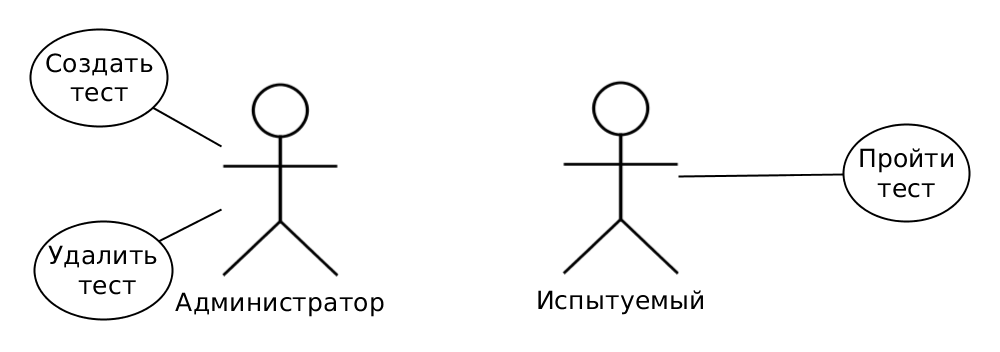
\includegraphics[width=0.8\textwidth]{img/usecase.png}
		\caption{Диаграмма вариантов использования}
		\label{uc:1}}
\end{figure}

\begin{sidewaysfigure}[!ht]
	\centering{ 
		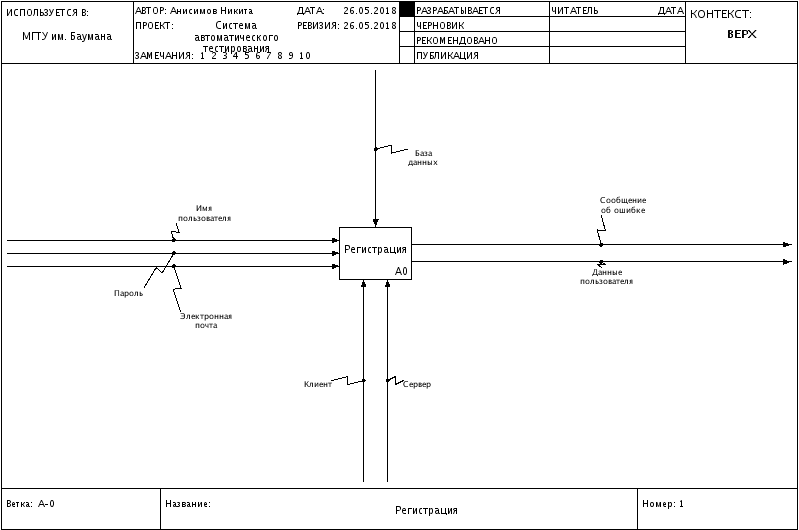
\includegraphics[width=0.8\textwidth]{img/reg_idef/01_A-0.png}
		\caption{Регистрация пользователя (уровень A0)}
		\label{idef0:00}}
\end{sidewaysfigure}
\begin{sidewaysfigure}[!ht]
	\centering{ 
		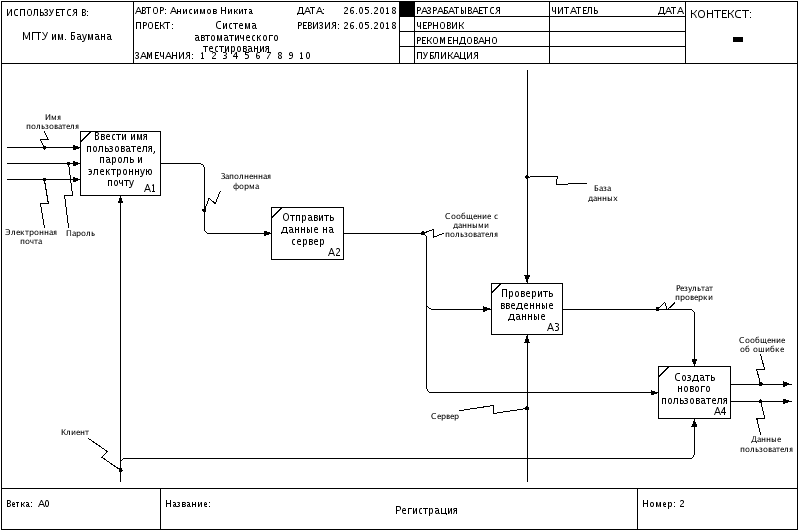
\includegraphics[width=0.8\textwidth]{img/reg_idef/02_A0.png}
		\caption{Регистрация пользователя (ветка А0)}
		\label{idef0:01}}
\end{sidewaysfigure}

\begin{sidewaysfigure}[!ht]
	\centering{ 
		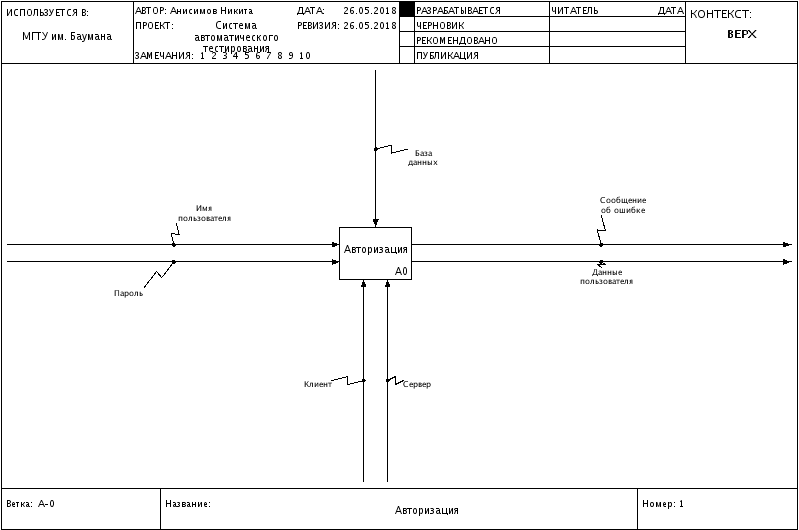
\includegraphics[width=0.8\textwidth]{img/authorzation_idef/01_A-0.png}
		\caption{Авторизация пользователя (уровень A0)}
		\label{idef0:10}}
\end{sidewaysfigure}
\begin{sidewaysfigure}[!ht]
	\centering{ 
		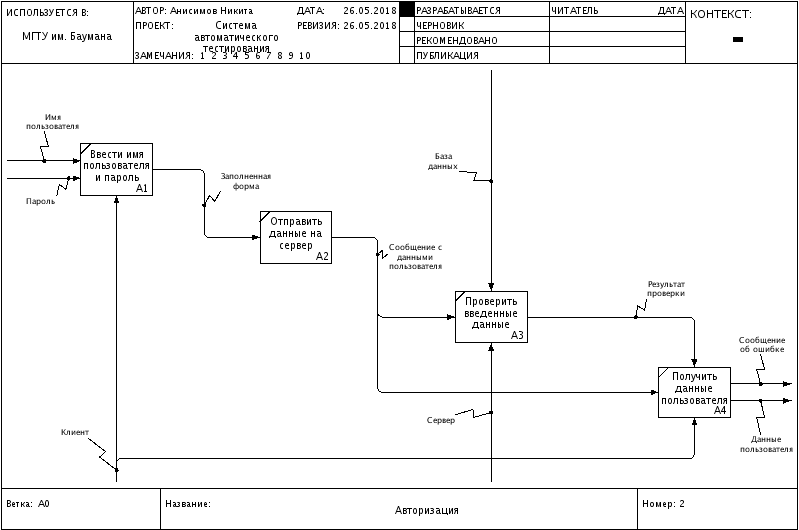
\includegraphics[width=0.8\textwidth]{img/authorzation_idef/02_A0.png}
		\caption{Авторизация пользователя (ветка А0)}
		\label{idef0:11}}
\end{sidewaysfigure}

\begin{sidewaysfigure}[!ht]
	\centering{ 
		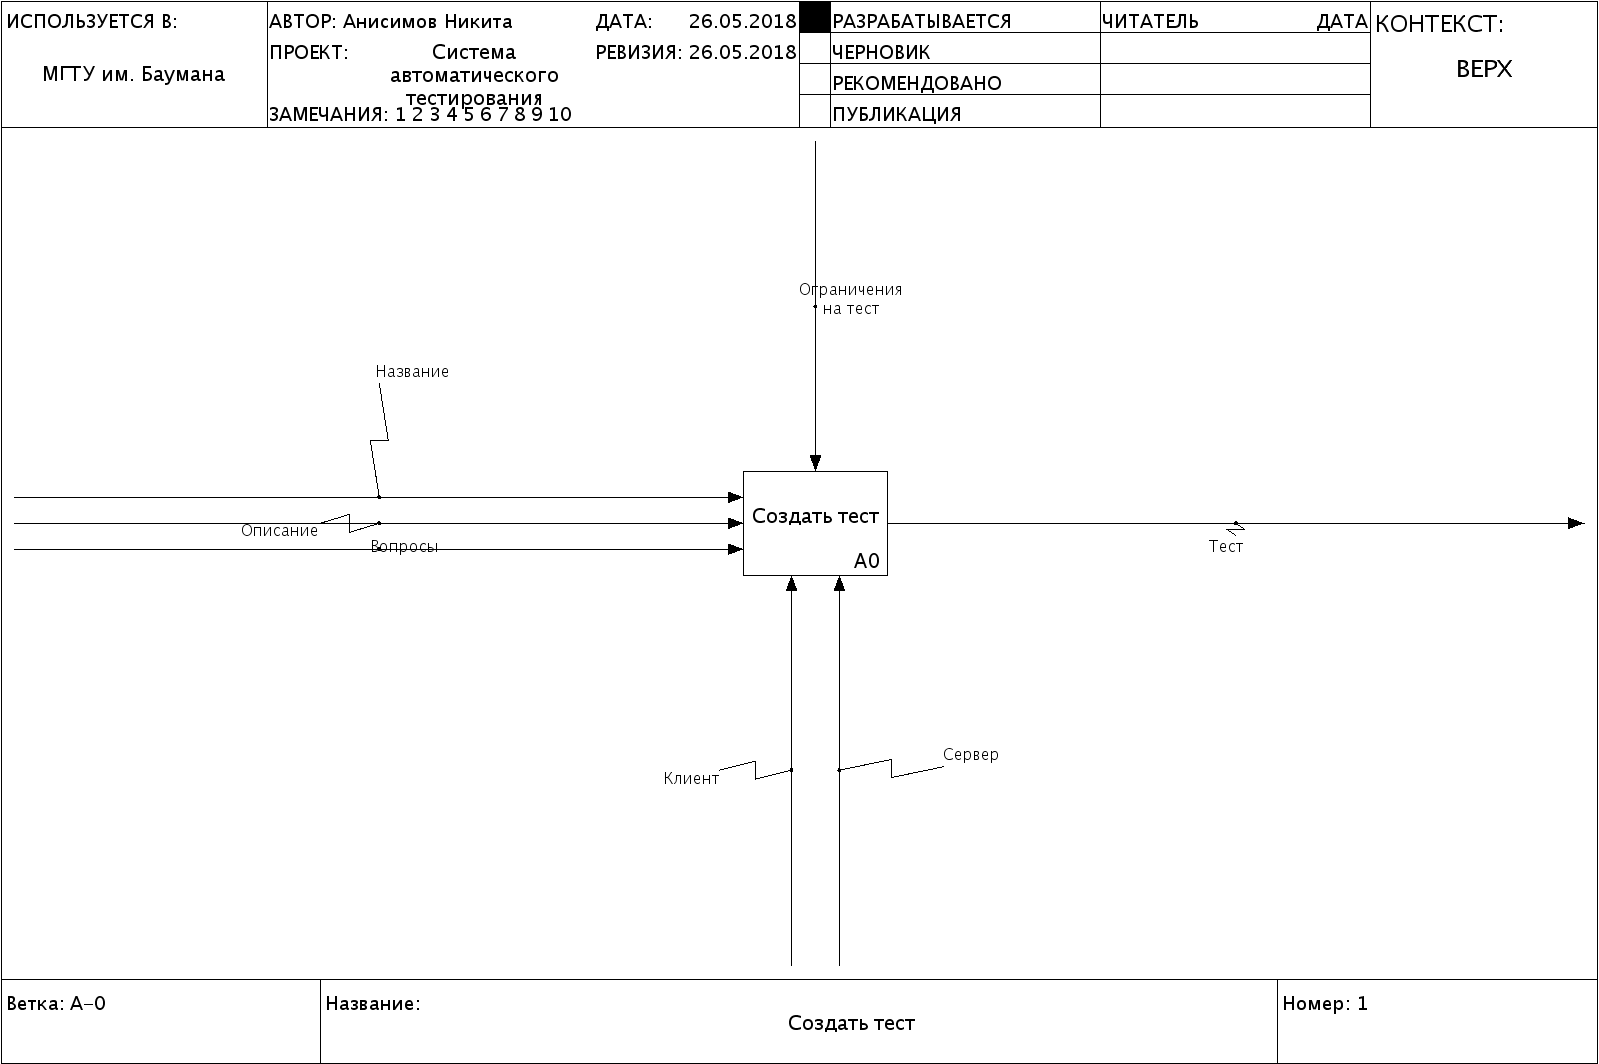
\includegraphics[width=0.8\textwidth]{img/new_idef/01_A-0.png}
		\caption{Создание теста (уровень A0)}
		\label{idef0:20}}
\end{sidewaysfigure}
\begin{sidewaysfigure}[!ht]
	\centering{ 
		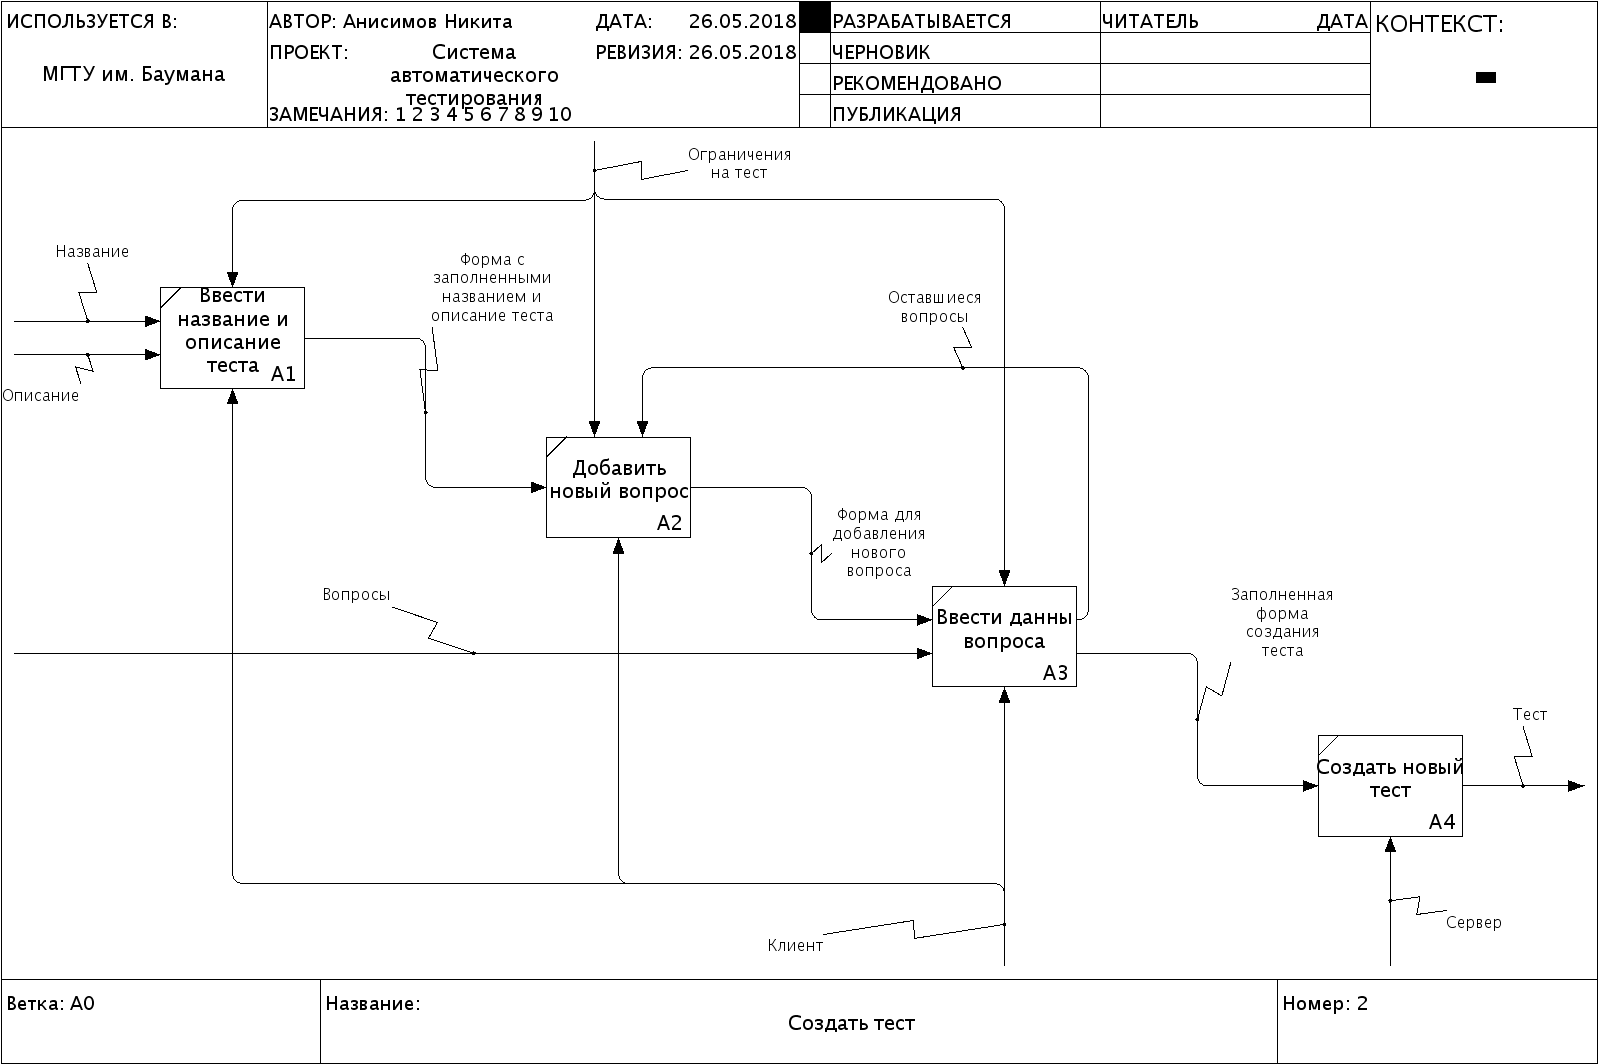
\includegraphics[width=0.8\textwidth]{img/new_idef/02_A0.png}
		\caption{Создание теста (ветка А0)}
		\label{idef0:21}}
\end{sidewaysfigure}


\begin{sidewaysfigure}[!ht]
	\centering{ 
		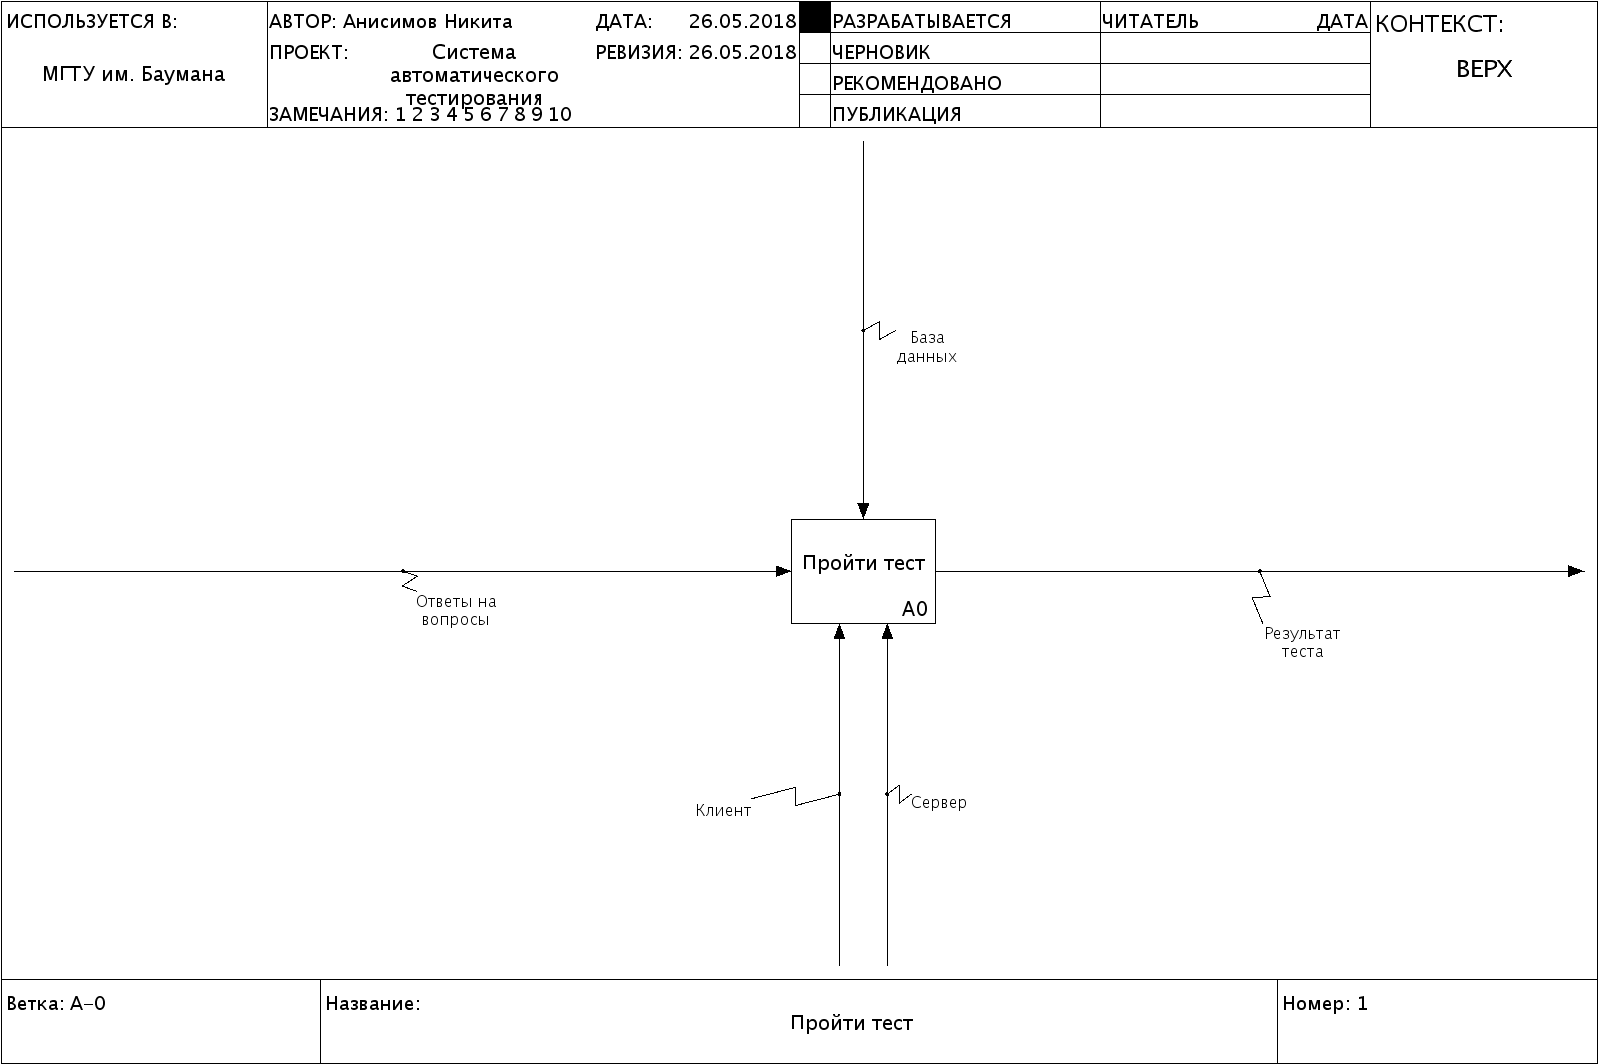
\includegraphics[width=0.8\textwidth]{img/pass_idef/01_A-0.png}
		\caption{Прохождение теста (уровень A0)}
		\label{idef0:30}}
\end{sidewaysfigure}
\begin{sidewaysfigure}[!ht]
	\centering{ 
		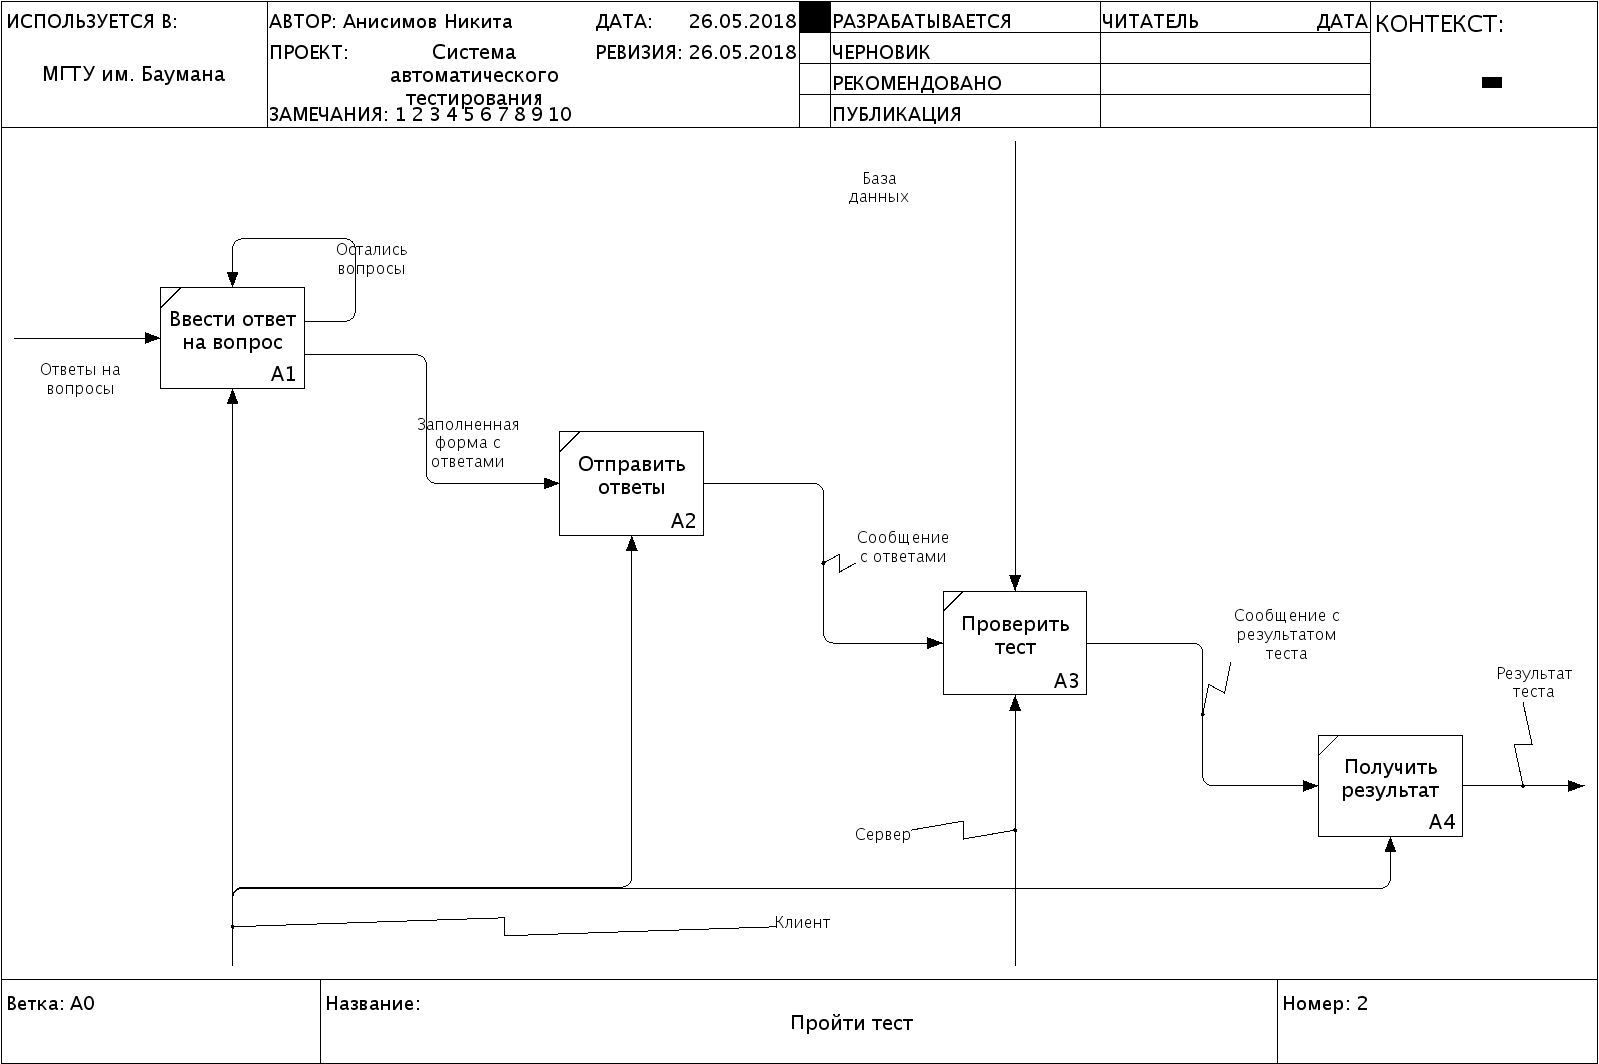
\includegraphics[width=0.8\textwidth]{img/pass_idef/02_A0.png}
		\caption{Прохождение теста (ветка А0)}
		\label{idef0:31}}
\end{sidewaysfigure}


\clearpage
\section{Разработка модели данных}

В результате анализа была выявлено 4 сущности: \texttt{Пользователь}, \texttt{Тест}, \texttt{Результат теста}, \texttt{Вопрос}.
\texttt{Пользователь} может создавать и проходить \texttt{Тесты}. После прохождения \texttt{Теста}, \texttt{Пользователь} получает новый \texttt{Результат теста}. В \texttt{Результате теста} хранится ключ на пройденный \texttt{Тест}. \texttt{Тест} содержит список \texttt{Вопросов}. ER-диаграмма данной модели представлена на рисунке \ref{er:1}.
\begin{figure}[ht!]
	\centering{ 
		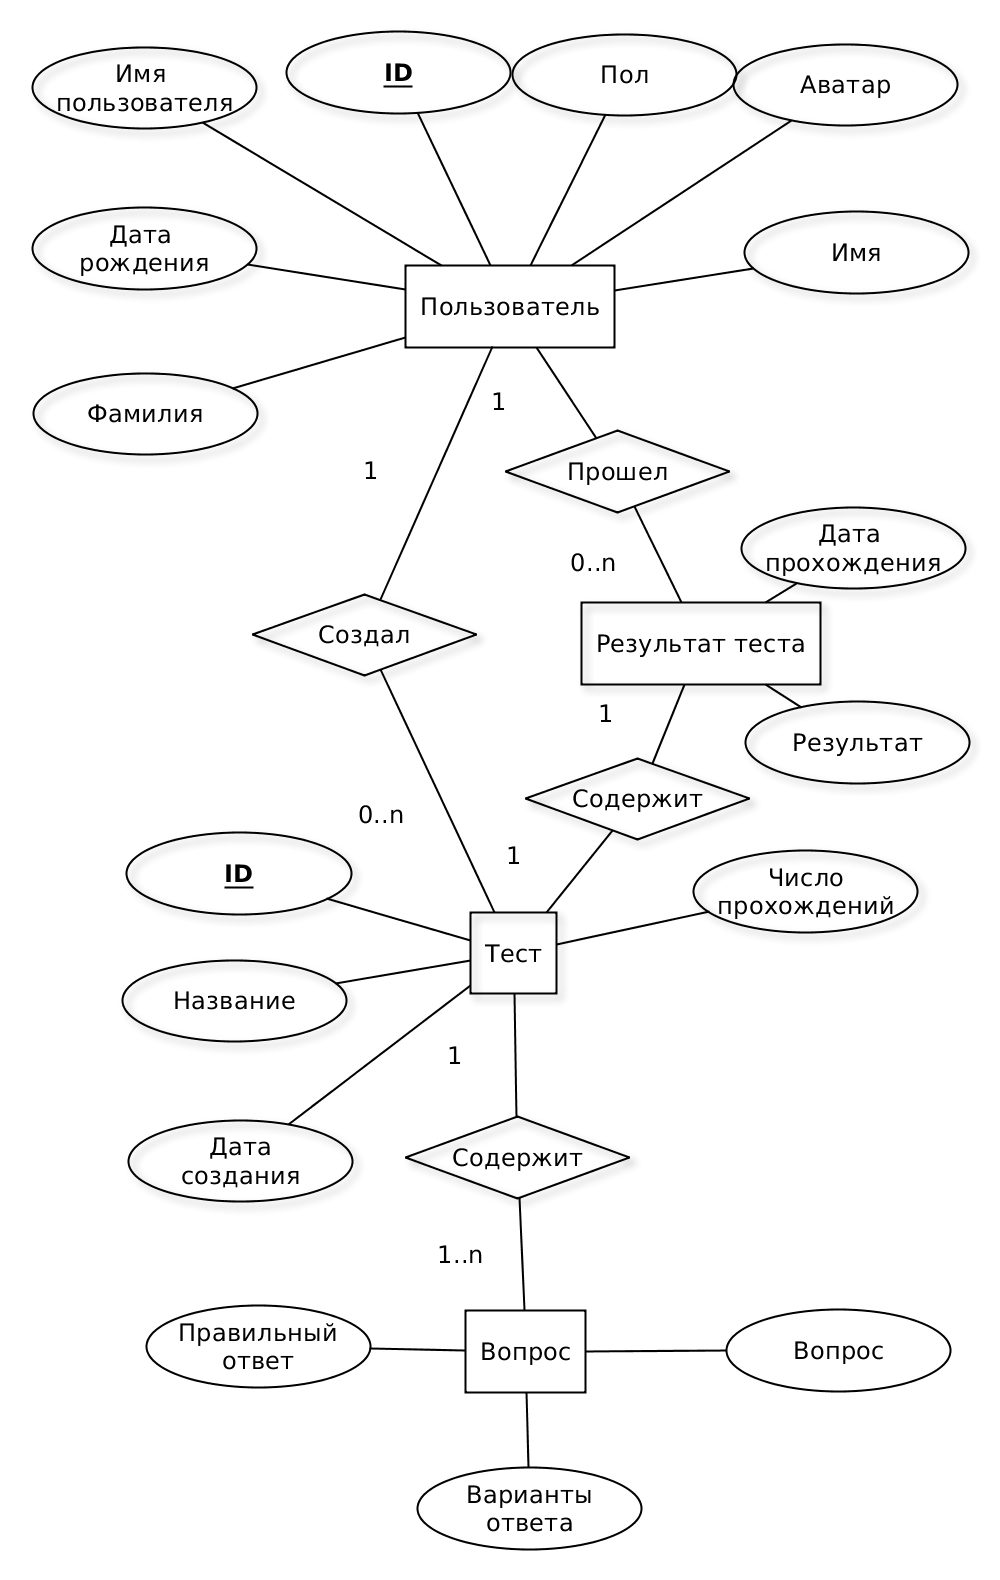
\includegraphics[width=0.7\textwidth]{img/er.png}
		\caption{ER-диаграмма (нотация Чена)}
		\label{er:1}}
\end{figure}

В качестве базы данных выбрана документоориентированная СУБД, благодаря чему становится возможным использование иерархических структур.

В таблицах \ref{user:doc} -- \ref{question:tbl} представлено описание каждой сущности.

\begin{table}[ht!]
	\centering
	\caption{Пользователь}
	\label{user:doc}
	\begin{tabular}{|l|l|l|}
		\hline
		\textbf{Поле} & \textbf{Тип}            & \textbf{Описание}                                                                                                                      \\ \hline
		username      &  Строка               & имя пользователя, уникально, не пусто                                                                                                             \\ \hline
		email         &  Строка               & электронная почта, уникально, не пусто                                                                                                            \\ \hline
		password      &  Строка               & \begin{tabular}[c]{@{}l@{}}пароль, не пусто, \\ не менее 8 символов\end{tabular}                                                       \\ \hline
		avatar        &  Строка               & \begin{tabular}[c]{@{}l@{}}путь до аватара пользователя, не пусто,\\ если аватара нет, путь до стандартного\\ изображения\end{tabular} \\ \hline
		first name    &  Строка               & имя, может быть пусто                                                                                                                  \\ \hline
		second name   &  Строка               & фамилия, может быть пусто                                                                                                              \\ \hline
		birthday      & Дата                    & \begin{tabular}[c]{@{}l@{}}дата рождения, может быть пусто,\\ не может быть больше сегодняшнего дня\end{tabular}                  \\ \hline
		gender        & Пол                     & пол, может быть пусто                                                                                                                  \\ \hline
		passed quiz   & Список<Тест>            & список тестов, может быть пусто                                                                                                        \\ \hline
		created quiz  & Список<Идентификатор>   & \begin{tabular}[c]{@{}l@{}}список ссылок на созданные тестов,\\ может быть пусто\end{tabular}                                          \\ \hline
	\end{tabular}
\end{table}

\begin{table}[ht!]
	\centering
	\caption{Результат теста}
	\label{quizResult:tbl}
	\begin{tabular}{|l|l|l|}
		\hline
		\textbf{Поле} & \textbf{Тип}  & \textbf{Описание}                   \\ \hline
		quiz id       & Идентификатор & ссылка на пройденный тест, не пусто \\ \hline
		result        &  Строка     & результат теста, не пусто           \\ \hline
		passing date  & Дата          & дата прохождения теста, не пусто    \\ \hline
	\end{tabular}
\end{table}

\begin{table}[ht!]
	\centering
	\caption{Тест}
	\label{quiz:tbl}
	\begin{tabular}{|l|l|l|}
		\hline
		\textbf{Поле}  & \textbf{Тип}   & \textbf{Описание}                \\ \hline
		name           &  Строка      & название теста, не пусто         \\ \hline
		description    &  Строка      & описание теста, не пусто         \\ \hline
		creation date  & Дата           & дата прохождения теста, не пусто \\ \hline
		passing number & Целое          & число сдач теста, не пусто       \\ \hline
		question       & Список<Вопрос> & список вопрос, не пусто          \\ \hline
	\end{tabular}
\end{table}

\begin{table}[ht!]
	\centering
	\caption{Вопрос}
	\label{question:tbl}
	\begin{tabular}{|l|l|l|}
		\hline
		\textbf{Поле} & \textbf{Тип}   & \textbf{Описание}                   \\ \hline
		text          &  Строка      & текст вопроса, не пусто             \\ \hline
		answer        &  Строка      & правильный вариант ответа, не пусто \\ \hline
		variants      & Список<Строка> & список вариантов ответа, не пусто   \\ \hline
	\end{tabular}
\end{table}

\section{Взаимодействие компонентов системы}

Взаимодействие компонентов системы представлено при помощи диаграмм последовательностей, изображенных на рисунках (\ref{seq:1}) -- (\ref{seq:10}). 

\begin{figure}[ht!]
	\centering{ 
		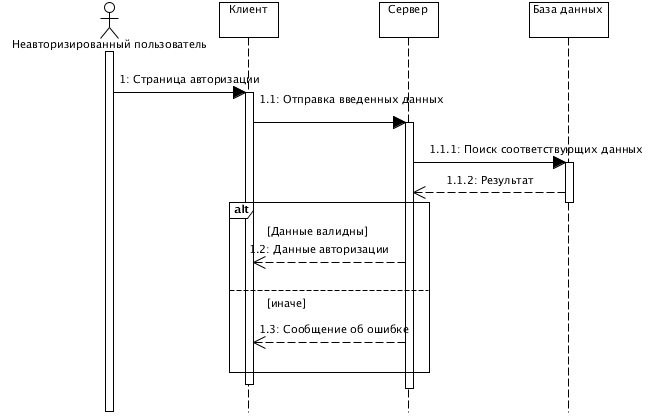
\includegraphics[width=1\textwidth]{img/sequence1.png}
		\caption{Взаимодействие компонентов при авторизации пользователей}
		\label{seq:1}}
\end{figure}
\begin{figure}[ht!]
	\centering{ 
		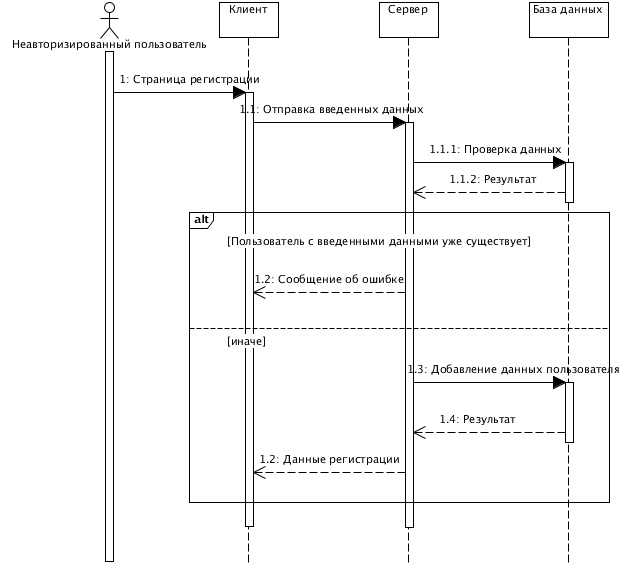
\includegraphics[width=1\textwidth]{img/sequence2.png}
		\caption{Взаимодействие компонентов при регистрации пользователей}
		\label{seq:2}}
\end{figure}
\begin{figure}[ht!]
\centering{ 
	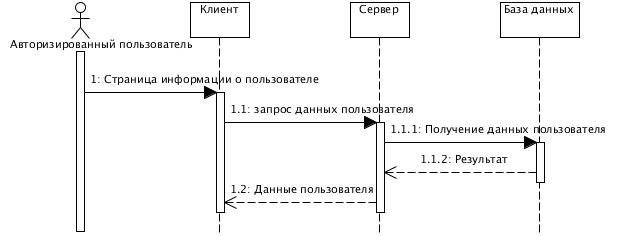
\includegraphics[width=1\textwidth]{img/sequence3.png}
	\caption{Взаимодействие компонентов при запросе данных пользователя}
	\label{seq:3}}
\end{figure}
\begin{figure}[ht!]
\centering{ 
	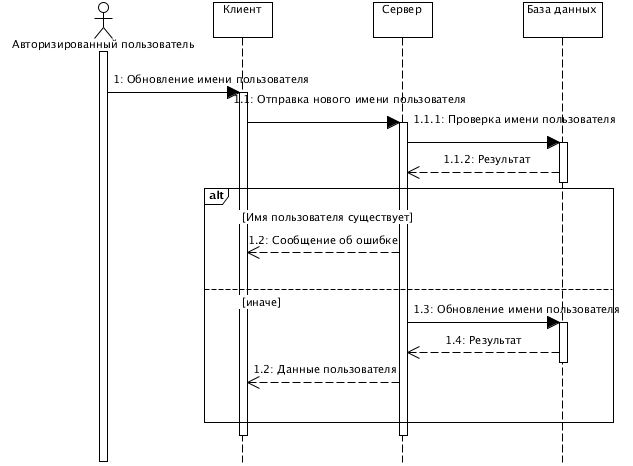
\includegraphics[width=1\textwidth]{img/sequence4.png}
	\caption{Взаимодействие компонентов при изменении имени пользователя}
	\label{seq:4}}
\end{figure}
\begin{figure}[ht!]
\centering{ 
	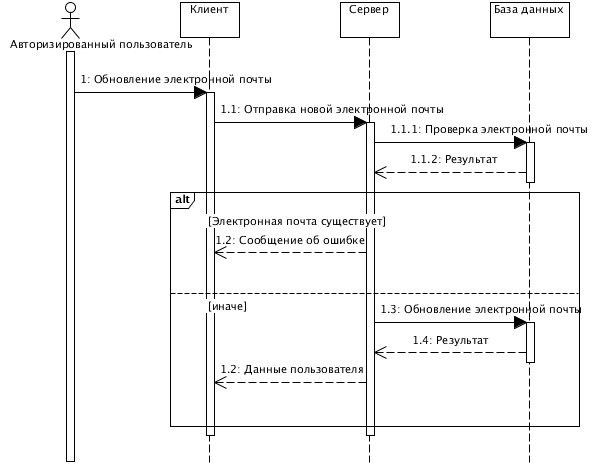
\includegraphics[width=1\textwidth]{img/sequence5.png}
	\caption{Взаимодействие компонентов при изменении электронной почты}
	\label{seq:5}}
\end{figure}
\begin{figure}[ht!]
\centering{ 
	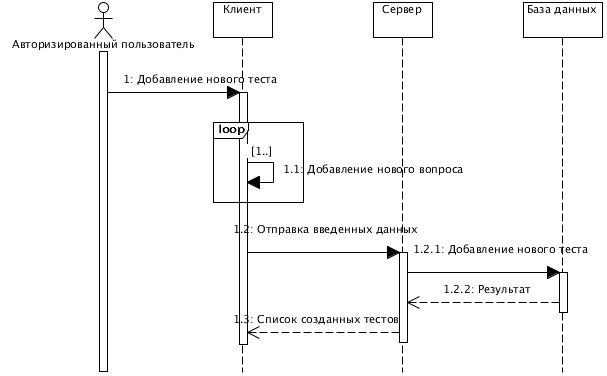
\includegraphics[width=1\textwidth]{img/sequence6.png}
	\caption{Взаимодействие компонентов при добавлении нового теста}
	\label{seq:6}}
\end{figure}
\begin{figure}[ht!]
	
\centering{ 
	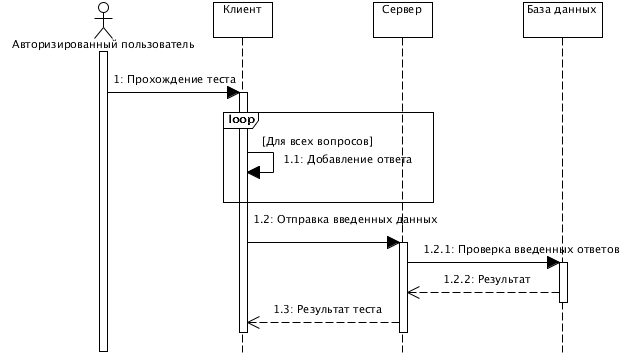
\includegraphics[width=1\textwidth]{img/sequence7.png}
	\caption{Взаимодействие компонентов при прохождении теста}
	\label{seq:7}}
\end{figure}
\begin{figure}[ht!]
\centering{ 
	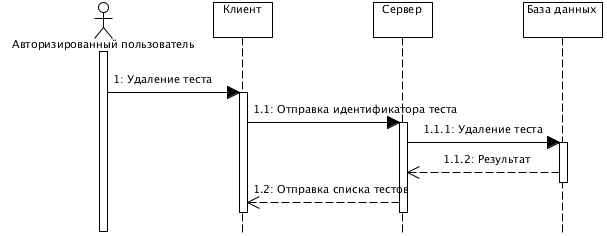
\includegraphics[width=1\textwidth]{img/sequence8.png}
	\caption{Взаимодействие компонентов при удалении теста}
	\label{seq:8}}
\end{figure}
\begin{figure}[ht!]
\centering{ 
	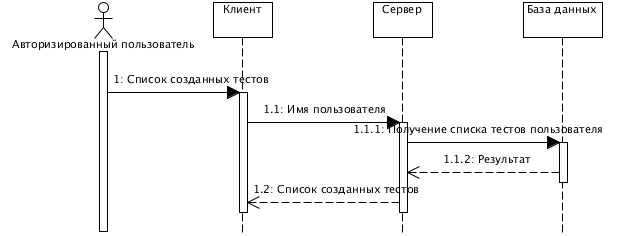
\includegraphics[width=1\textwidth]{img/sequence9.png}
	\caption{Взаимодействие компонентов при получении списка созданных пользователем тестов}
	\label{seq:9}}
\end{figure}
\begin{figure}[ht!]
\centering{ 
	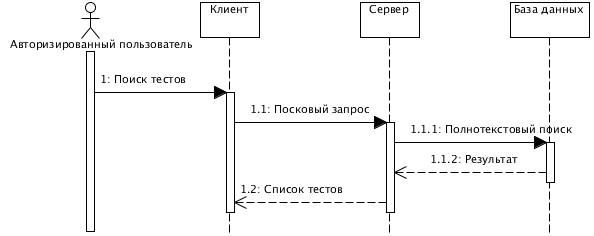
\includegraphics[width=1\textwidth]{img/sequence10.png}
	\caption{Взаимодействие компонентов при поиске тестов}
	\label{seq:10}}
\end{figure}
\chapter{Технологический раздел}
На сегодняшний день существует большое количество языков и технологий, используемых как для разработки серверной части, так и для клиентской части.
\section{Сервер}

\subsection{База данных}
В качестве базы данных была выбрана NoSQL база данных MongoDB.

MongoDB это кросс-платформенная, документоориентированная база данных, которая обеспечивает высокую производительность и лёгкую масштабируемость. В основе данной СУБД лежит концепция коллекций и документов.

Коллекция – это группа документов MongoDB. Является эквивалентом простой таблицы в реляционной базе данных. Коллекция помещена внутри одной БД. Документ в коллекции может иметь различные поля. Чаще всего, все документы в коллекции созданы для одной, либо относящихся друг ко другу целей.

Документ – это набор пар <<ключ – значение>>. Документ имеет динамическую схему. Это означает, что документ в одной и той же коллекции не обязан иметь один одинаковый набор полей или структуру, а общие поля в коллекции могут иметь различные типы данных.

Любая реляционная БД имеет стандартную схему, которая показывает количество таблиц и связи между ними. В MongoDB такой схемы с связи между таблицами нет.

Основные особенности MongoDB:

\begin{itemize}
	\item Отсутствие схемы.
	\item Данная БД основана на коллекциях различных документов. Количество полей, содержание и размер этих документов может отличаться. Т.е. различные сущности не должны быть идентичны по структуре.
	\item Легко масштабируется.
	\item Для хранения используемых в данный момент данных используется внутренняя память, что позволяет получать более быстрый доступ.
	\item Данные хранятся в виде JSON документов.
	\item MongoDB поддерживает динамические запросы документов (document-based query).
	\item Отсутствие сложных JOIN запросов.
\end{itemize}

\subsection{Язык}
В качестве языка программирование для разработки серверной части был выбран язык Haskell. 

Haskell – это функциональный язык. Он воплощает понятие чистоты, модель его вычислений основана на концепции “лени”, обладает параметрическим полиморфизмом. 

Среди особенностей данного языка можно отметить следующие:
\begin{itemize}
	\item \textbf{Автоматическое управление памятью.} Память выделяется неявно, автоматически, а специальный сборщик мусора (garbage collector) возвращает системе неиспользуемые куски памяти. Оптимальные алгоритмы управления памятью сложны, но сегодня уже достаточно хорошо проработаны. Использование этих алгоритмов не сильно увеличивают время работы программы в целом (в сравнении с тем, когда программист сам, по-умному, занимается выделением и освобождением памяти).
	
	\item \textbf{Чистые функции.} Функция называется детерминированной, если возвращаемое ею значение зависит только от аргументов. Говорят, что функция не имеет побочных эффектов, если при ее вызове не производится запись в файл, чтение из сокета, изменение глобальных переменных и так далее. Функция называется чистой, если она является детерминированной и не имеет побочных эффектов. Все функции в Haskell представляют собой выражения, подобные математическим. Они не имеют побочных эффектов (за некоторыми исключениями). Работа с сетью и файлами производится посредством <<грязных>> функций. В Haskell функции поделены на чистые и <<грязные>>, то есть недетерминированные и имеющие побочные эффекты. <<Грязные>> функции используются для ввода данных, передачи их в чистые функции и вывода результата.
	
	\item \textbf{Ленивая модель вычислений.} Haskell реализует ленивую модель вычислений. Выражение на языке Haskell – это лишь обещание того, что оно будет вычислено при необходимости. Одной из проблем ленивых вычислений является использование большого количества памяти, так как необходимо хранить целое выражение для последующего вычисления. Поскольку большинство функций в Haskell являются чистыми, значения, возвращаемые функцией для заданных аргументов, кэшируются. Если функция вызывается многократно с одними и теми же аргументами, реальная работа выполняется только один раз. При втором или третьем вызове из кэша берется уже посчитанное значение.
	
	\item \textbf{Параметрический полиморфизм.} Параметрический полиморфизм позволяет давать участку кода обобщенный тип, используя переменные вместо настоящих типов, а затем конкретизировать, замещая переменные типами. Параметрические определения однородны: все экземпляры данного фрагмента кода ведут себя одинаково.
	
	\item \textbf{Параллельные вычисления.} Haskell обеспечивает программиста средствами детерминированного параллельного программирования. Они позволяют ускорить чистое вычисление, не теряя при этом самой чистоты.
	
	\item \textbf{Широкая область применения.} Существует большое количество программ, написанных на языке Haskell, от приложений с графическим интерфейсом, до серверов.
	
	 
\end{itemize}

\subsection{Servant}
Фреймворк -- программная платформа, определяющая структуру программной системы; программное обеспечение, облегчающее разработку и объединение разных компонентов большого программного проекта.

Servant -- это веб-фреймворк, для языка Haskell. Одним из основных преимуществ данного фреймворка заключается в том, что API сервера описывается как тип. Таким образом на этапе компиляции могут быть отловлены все несоответствия со спецификацией API.

Описание API выглядит следующим образом: 
\lstinputlisting[caption = {Определение API}, label={lst3:label},language=Haskell, firstline=11, lastline=38]{../Server/src/API/User/API.hs}

\subsection{Persistent}
Haskell предлагает множество различных библиотек к базам данных. Однако большинство из них имеют малое представление о схеме базы данных и потому не обеспечивают полезных статических проверок. Кроме того, они вынуждают программиста использовать API и типы данных, зависящие от конкретной базы данных. Чтобы избавиться от этих проблем, программистами на Haskell была предпринята попытка пойти более революционным путем и создать хранилище данных, специфичное для Haskell, тем самым получив возможность с легкостью хранить любой тип данных Haskell. Эта возможность действительно прекрасна в некоторых случаях, но она делает программиста зависимым от техники хранения данных и используемой библиотеки, плохо взаимодействует с другими языками, а также для обеспечения гибкости может требовать от программиста написания большого количества кода, запрашивающего данные. В отличие от Persistent, который предоставляет выбор среди множества баз данных, каждая из которых оптимизирована для различных случаев, позволяет взаимодействовать с другими языками, а также использовать безопасный и производительный интерфейс запросов.

Persistent следует принципам безопасности типов и краткого, декларативного синтаксиса. Среди других возможностей следует отметить:

\begin{itemize}
	\item Независимость от базы данных. Имеется первоклассная поддержка PostgreSQL, SQLite и MongoDB, а также экспериментальная поддержка CouchDB и находящаяся в разработке поддержка MySQL.
	\item Будучи нереляционным по своей природе, Persistent позволяет одновременно поддерживать множество слоев хранения данных и не обременен проблемами производительности, связанными с использованием JOIN’ов.
	\item Основной проблемой при использовании SQL баз данных является попытка изменения схемы базы данных. Persistent позволяет автоматически выполнять обновление схемы базы данных.
\end{itemize}

Пакет Persistent активно использует расширение языка Template Haskell. Template Haskell (TH) — это расширение Haskell, добавляющее в язык шаблоны. Шаблоны в Haskell представляют собой подобие макросов Lisp, только со строгой статической типизацией. Другими словами, TH добавляет в язык возможность метапрограммирования, то есть, написания программ, которые генерируют код программы на этапе компиляции. 

\subsection{Создание коллекций}
Коллекции создаются описанием моделей данных на специальном синтаксисе, предоставляемом библиотекой Persistent. Код создания моделей представлен в листинге \ref{lst1:label}.

В качестве типа при описании поля модели используется тип языка Haskell. В таблице \ref{tbl1} представлено соответствие между типами языка Haskell и базы данных MongoDB.

Для указания того, что поле может содержать значение \texttt{null} или отсутствовать, используется слово \texttt{Maybe}. Чтобы использовать внешний ключ на какую либо объявленную модель, в качестве типа данных указывается тип \texttt{\{Модель\}Id}, где \texttt{\{Модель\}} -- это одна имя одной из объявленных моделей. Например, модели \texttt{QuizResult} и \texttt{User} имеют внешний ключ на модель \texttt{Quiz}, и в качестве типа поля используют \texttt{QuizId}. 

Для реализации иерархической структуры в качестве типа указывается тип Модели. Модель \texttt{Quiz} включает в себя список вопросов \texttt{Question}, а модель \texttt{User} включает в себя список пройденных тестов \texttt{QuizResult}.

\begin{table}[]
	\centering
	\caption{Соответствие между типами языка Haskell и базы данных MongoD}
	\label{tbl1}
	\begin{tabular}{|l|l|}
		\hline
		\textbf{Haskell} & \textbf{MongoDB}     \\ \hline
		Text             & String               \\ \hline
		ByteString       & BinData              \\ \hline
		Int              & NumberLong           \\ \hline
		Double           & Double               \\ \hline
		Rational         & \textit{Unsupported} \\ \hline
		Bool             & Boolean              \\ \hline
		Day              & NumberLong           \\ \hline
		TimeOfDay        & \textit{Unsupported} \\ \hline
		UTCTime          & Date                 \\ \hline
	\end{tabular}
\end{table}

\lstinputlisting[caption = {Определение моделей}, label={lst1:label},language=Haskell, firstline=29, lastline=64]{../Server/src/Model/Model.hs}

Поле \texttt{\_id} создается автоматически базой данных MongoDB для каждой коллекции и имеет индекс Primary Key. 


\subsection{Создание индексов коллекции \texttt{user}}
Поля \texttt{username} и \texttt{email} коллекции \texttt{user} должны быть уникальными, поэтому для них необходимо создать ограничение уникальности. 
Библиотека Persistent не содержит функции создания индексов, поэтому в данном случае необходимо воспользоваться функцией библиотеки mongodb.

\lstinputlisting[caption = {Создание уникальных индексов}, label={lst2:label},language=Haskell, firstline=71, lastline=74]{../Server/src/Model/Model.hs}

\subsection{Создание индексов коллекции \texttt{quiz}}
Полнотекстовый поиск должен производиться по полям \texttt{name} и \texttt{description}. Для этого необходимо создать соответствующий индекс.
В данном случае, ни одна из используемых библиотек не поддерживает создание индекса полнотекстового поиска, поэтому необходимо создать документ с необходимыми параметрами индекса, и включить его в системную таблицу \texttt{system.indexes}.

\lstinputlisting[caption = {Создание индекса для полнотекстового поиска}, label={lst2:label},language=Haskell, firstline=77, lastline=89]{../Server/src/Model/Model.hs}


\subsection{Описание методов API}

\request{POST} {/user/login}
{Авторизация пользователя}
{<объект авторизации>}
{<JWT токен>}
{\status{200} \sep \status{404} \sep \status{500}}

\request{POST} {/user/register}
{Регистрация пользователя}
{<объект регистрации>}
{<JWT токен>}
{\status{200} \sep \status{400} \sep \status{500}}

\request{GET} {/user/username}
{Получение имени пользователя}
{}
{<Строка>}
{\status{200} \sep \status{401} \sep \status{500}}


\request{GET} {/user/profile}
{Получение информации о пользователе}
{}
{<объект профиля пользователя>}
{\status{200} \sep \status{401} \sep \status{500}}



\request{POST} {/user/edit/username}
{Изменение имени пользователя}
{строка}
{<JWT токен>}
{\status{200} \sep \status{401} \sep \status{500}}


\request{POST} {/user/edit/password}
{Изменение пароля}
{<строка>}
{}
{\status{200} \sep \status{401} \sep \status{500}}

\request{POST} {/user/edit/email}
{Изменение электронной почты пользователя}
{<строка>}
{}
{\status{200} \sep \status{401} \sep \status{500}}

\request{POST} {/user/edit/avatar}
{Изменение картинки пользователя}
{<изображение>}
{<строка>}
{\status{200} \sep \status{401} \sep \status{500}}

\request{POST} {/user/edit/profile}
{Изменение информации о пользователе}
{<объект профиля пользователя>}
{}
{\status{200} \sep \status{401} \sep \status{500}}


\request{POST} {/quiz/new}
{Добавление нового теста}
{<объект теста>}
{}
{\status{200} \sep \status{401} \sep \status{500}}

\request{GET} {/quiz/get/user/{offset}/{count}}
{Получение \{count\} тестов, созданных пользователем, начиная с \{offset\}}
{}
{<список объектов теста>}
{\status{200} \sep \status{401} \sep \status{500}}

\request{GET} {/quiz/get/{offset}/{count}}
{Получение \{count\} тестов, начиная с \{offset\}}
{}
{<список объектов теста>}
{\status{200} \sep \status{401} \sep \status{500}}

\request{GET} {/quiz/get/{id}}
{Получение конкретного теста, с заданным \{id\}}
{}
{<объекта теста>}
{\status{200} \sep \status{401}\sep \status{404}  \sep \status{500}}

\request{GET} {/quiz/search/{query}/{offset}/{count}}
{Получение \{count\} тестов, начиная с \{offset\}, удовлетворяющих запросу \{query\}}
{}
{<список объектов теста>}
{\status{200} \sep \status{401} \sep \status{500}}

\request{POST} {/quiz/remove/{id}}
{Удаление теста с заданным \{id\}}
{}
{}
{\status{200} \sep \status{401}\sep  \status{404}   \sep \status{500}}

\request{POST} {/quiz/result/{id}}
{Добавление результатов теста, с заданным \{id\}}
{<объект результата теста>}
{}
{\status{200} \sep \status{401}\sep  \status{404}   \sep \status{500}}

\section{Клиент}

Клиент был разработан на языке Elm. 

Elm — функциональный язык, предназначенный для декларативного создания графических интерфейсов, основанных на браузере. Elm предоставляет возможность описывать графические интерфейсы, не выходя за рамки функциональной парадигмы, используя функционально-реактивный стиль программирования.

Изначальная реализация компилировала Elm в HTML, CSS и JavaScript. В следующих выпусках набор инструментов был расширен: добавлен REPL, пакетный менеджер, отладчик и установщики для Mac OS и Windows. На официальном сайте ведётся репозиторий библиотек, разрабатываемых для языка.

Язык обладает следующими особенностями:
\begin{itemize}
	\item Код на языке Elm компилируется в JavaScript код.
	\item Elm код не производит ошибок во время выполнения. Elm использует вывод типов для обнаружения проблем во время компиляции.
	\item Высокая производительность по сравнению с другими фронт-энд фреймворками.
\end{itemize}

Логика любой программы на Elm, делится на три части:
\begin{itemize}
	\item Модель -- состояние приложения.
	\item Обновление -- способ обновления состояния.
	\item Представление -- способ отображения состояния как HTML.
\end{itemize}

Каждое приложение имеет следующий общий вид:
\begin{lstlisting}
import Html exposing (..)

-- Модель

type alias Model = { ... }

-- Обновление

type Msg = Reset | ...

update : Msg -> Model -> Model
update msg model =
case msg of
Reset -> ...
...

-- Представление

view : Model -> Html Msg
view model =
...
\end{lstlisting}

\section{Интерфейс}
На рисунках (\ref{scr1}) -- (\ref{scr4}) представлен интерфейс некоторых страниц системы.

\begin{figure}[ht!]
	\centering{ 
		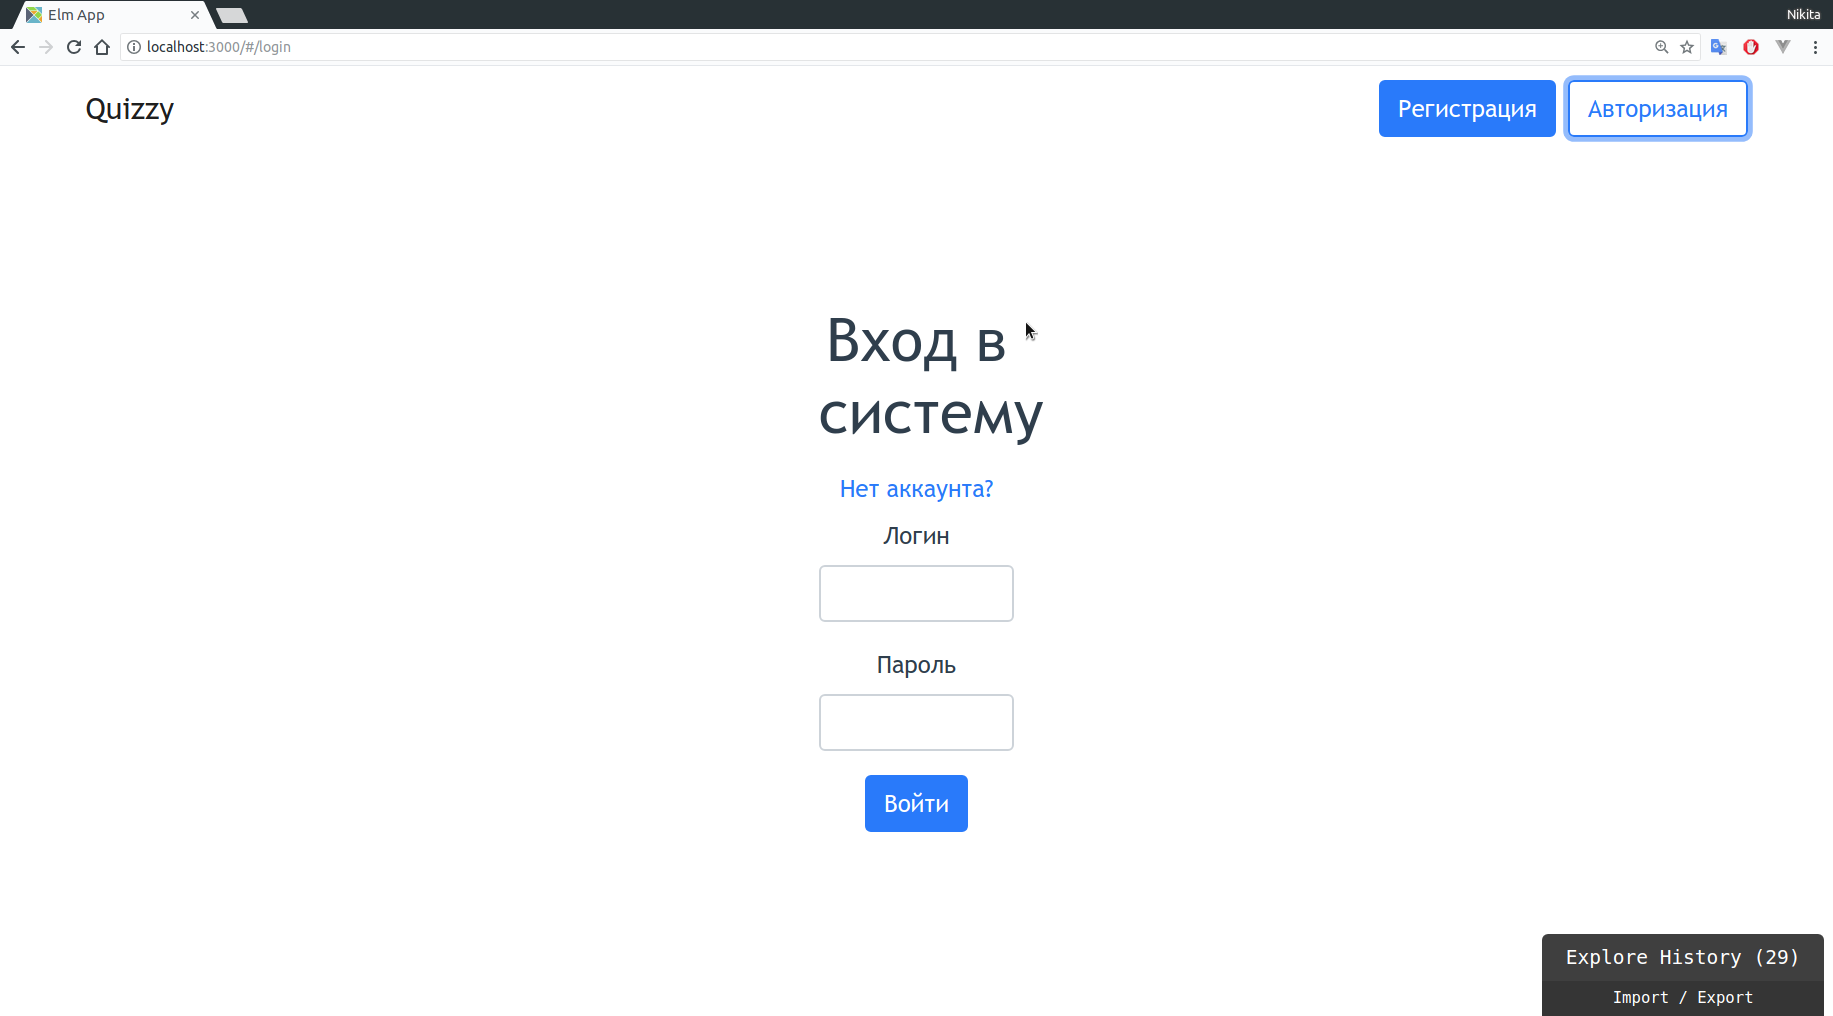
\includegraphics[width=1\textwidth]{img/screens/auth.png}
		\caption{Страница авторизации пользователя}
		\label{scr1}}
\end{figure}
\begin{figure}[ht!]
	\centering{ 
		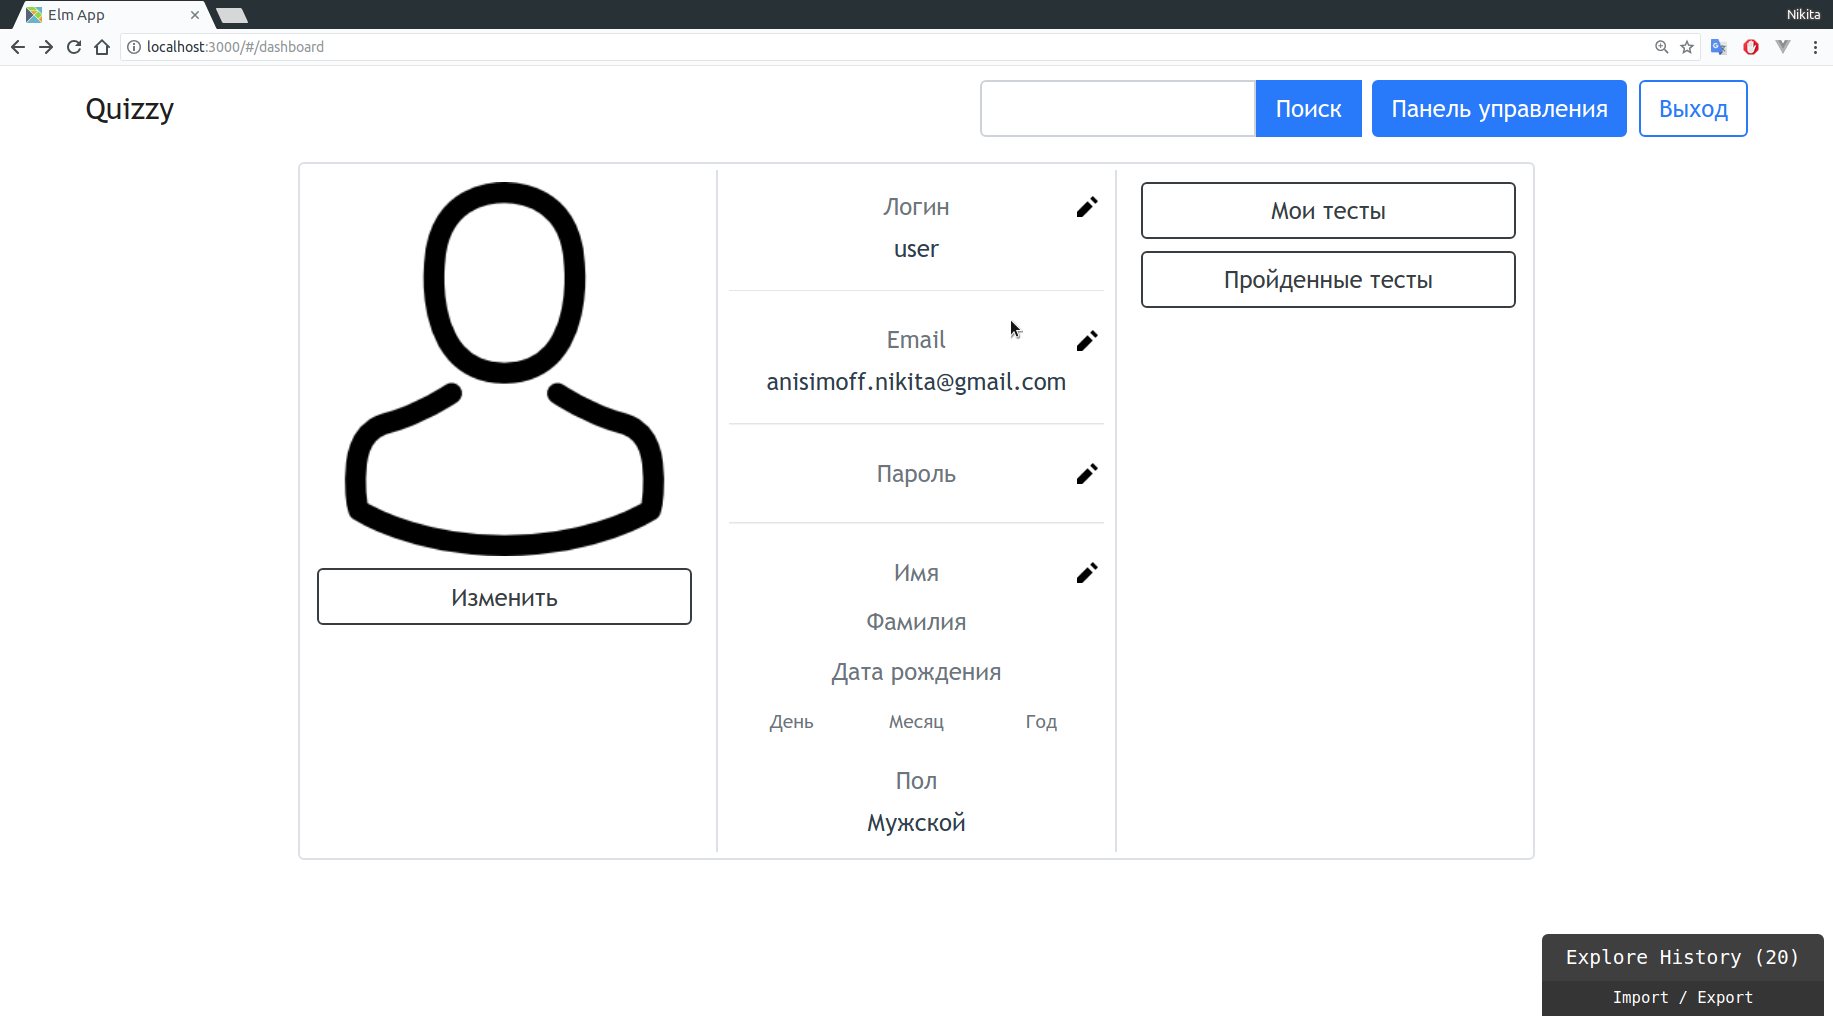
\includegraphics[width=1\textwidth]{img/screens/db.png}
		\caption{Страница пользователя}
		\label{scr2}}
\end{figure}
\begin{figure}[ht!]
	\centering{ 
		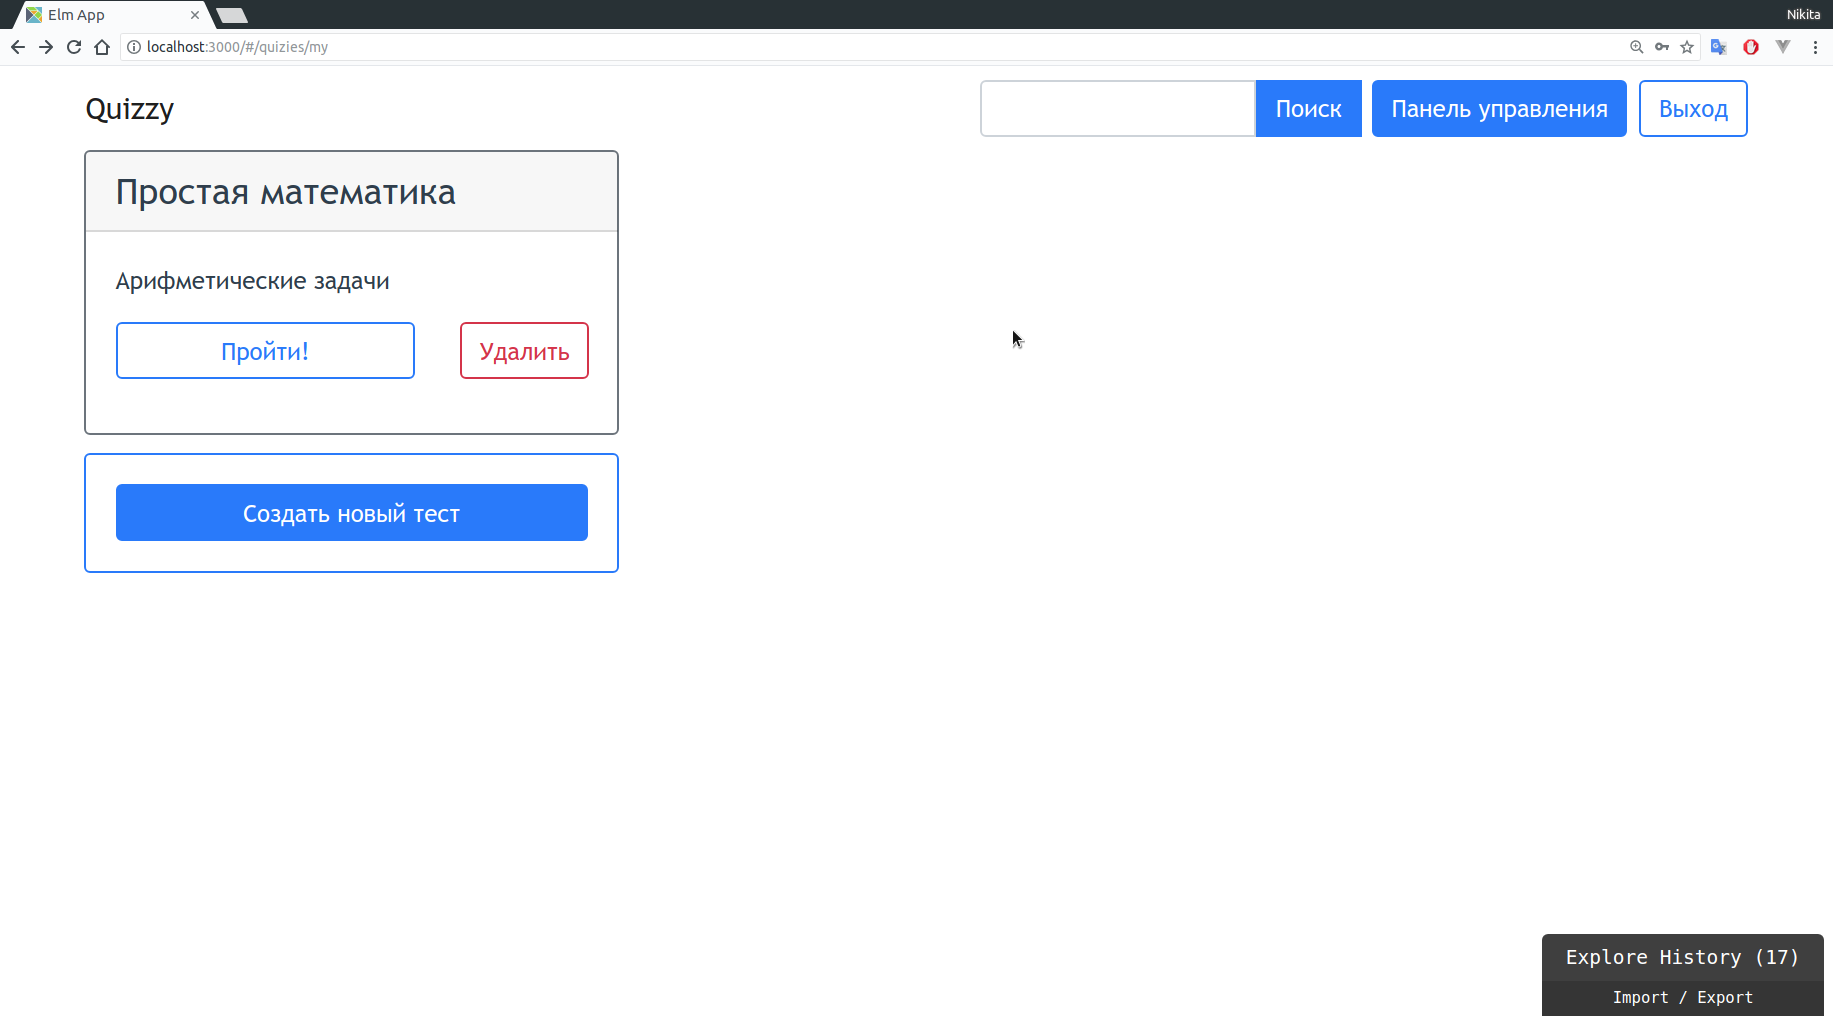
\includegraphics[width=1\textwidth]{img/screens/list.png}
		\caption{Страница управления тестами}
		\label{scr3}}
\end{figure}
\begin{figure}[ht!]
	\centering{ 
		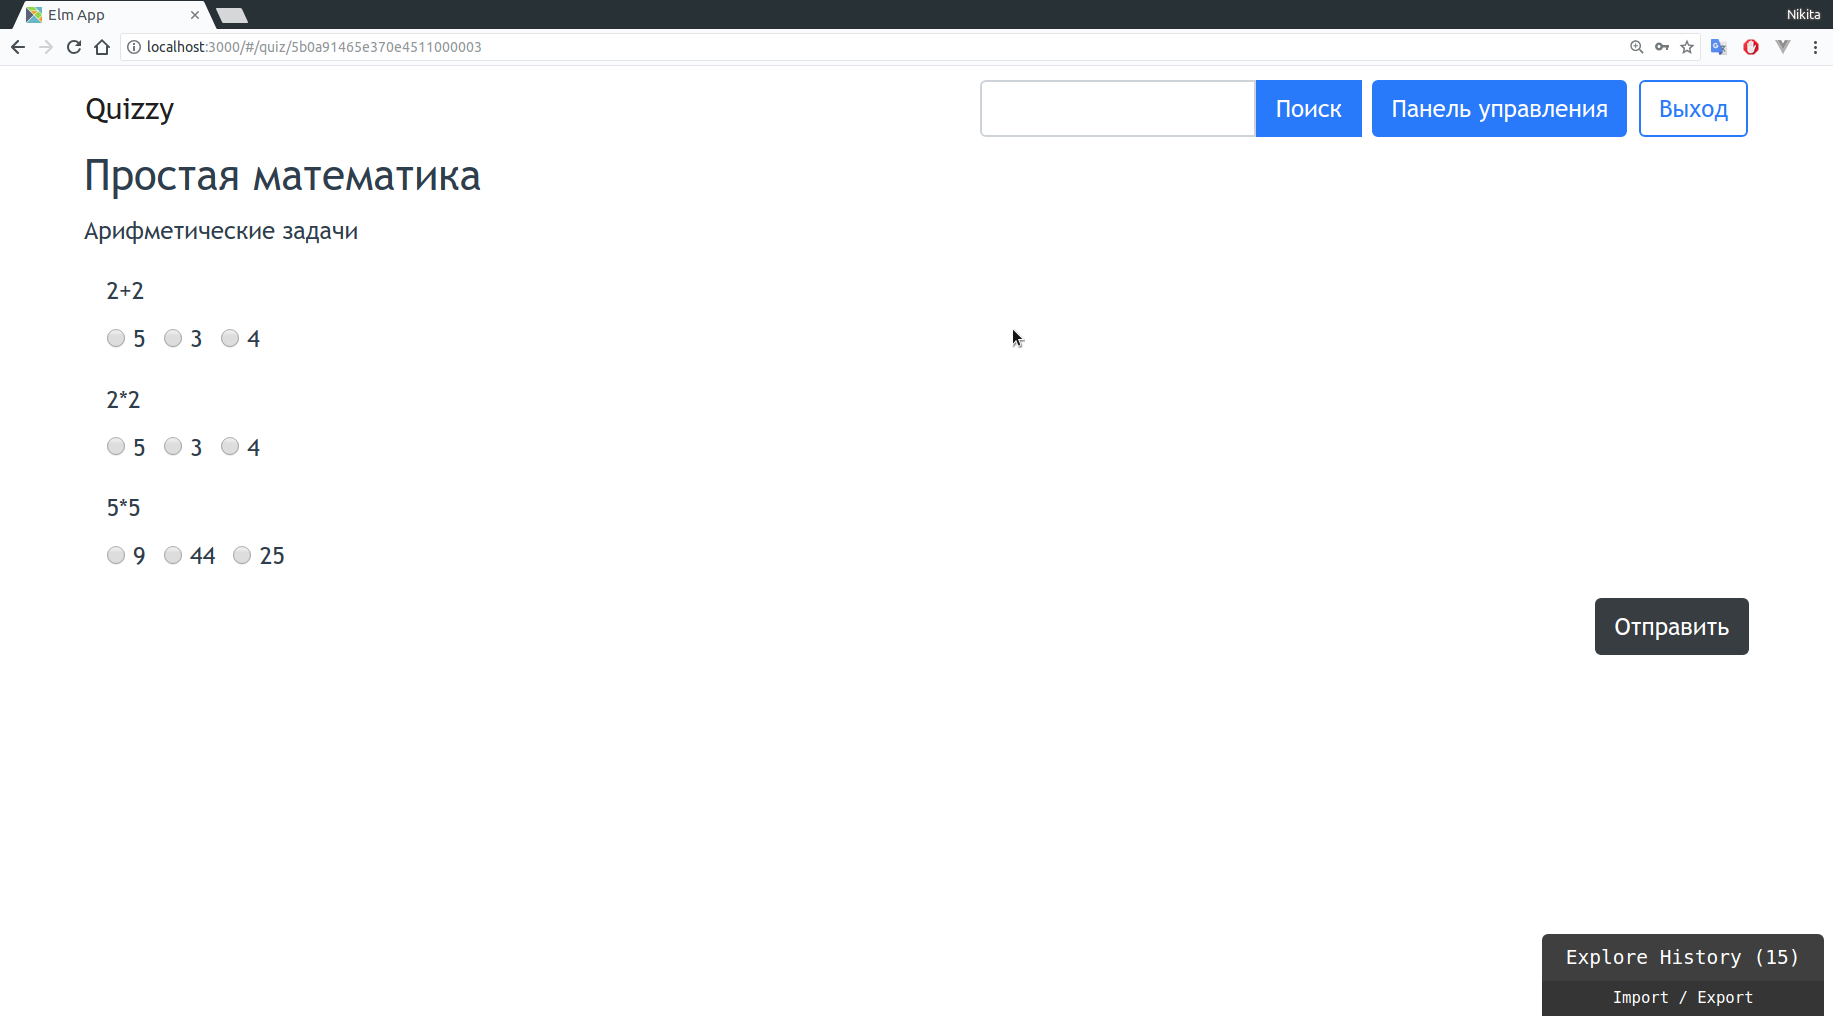
\includegraphics[width=1\textwidth]{img/screens/pass.png}
		\caption{Страница прохождения теста}
		\label{scr4}}
\end{figure}

\clearpage
\section{Выводы}
В качестве документооринтированной базы данных была выбрана MongoDB. Серверная часть написана на языке Haskell, с использованием библиотек Servant и Persistent. Клиент написан на языке Elm. Система разработана и протестирована.
%\include{5-expiremental}

\backmatter %% Здесь заканчивается нумерованная часть документа и начинаются ссылки и

\chapter{Заключение}
В ходе данной работы была разработана автоматической тестирующей системы. Пользователь имеет возможность создавать и проходить тесты.

Определены роли пользователей: администратор -- создает тесты, и испытуемый -- выполняет задания. 

Детально были описаны процесса авторизации, регистрации, добавления и прохождения тестов с использование IDEF0 диаграмм. 

Выявлены следующие сущности: \texttt{Пользователь}, \texttt{Тест}, \texttt{Результат теста}, \texttt{Вопрос}. Пользователь создает и проходит тесты. Тесты содержат вопросы. В результате выполнения теста, пользователь получает результат теста. Для данных сущностей построена ER-диаграмма. Описаны и документированы атрибуты каждой сущности.

С помощью диаграмм последовательностей описаны взаимодействия системы в следующих действиях: авторизация, регистрация, запрос данных пользователя, изменение имени пользователя, изменение пароля пользователя, изменение электронной почты пользователя, добавление нового теста, прохождение теста, удаление теста, получение списка созданных тестов, поиск тестов.

В качестве базы данных выбрана нерялиционная документооринетированная база данных MongoDB. Были описаны преимуществе данной БД.

Для разработки серверной части использовался язык Haskell. В качестве веб-фреймворка использовалась библиотека Servant. Пакет Persistent использовался для взаимодействия с базой данных. Клиентская часть разработана на языке Elm.

            %% заключение

%\include{60-conclusion}

%\include{61-biblio}

%\appendix   % Тут идут приложения

%\include{90-appendix1}
%\include{91-appendix2}

\end{document}

%%% Local Variables:
%%% mode: latex
%%% TeX-master: t
%%% End:
